\PassOptionsToPackage{unicode=true}{hyperref} % options for packages loaded elsewhere
\PassOptionsToPackage{hyphens}{url}
%
\documentclass[]{article}
\usepackage{lmodern}
\usepackage{amssymb,amsmath}
\usepackage{ifxetex,ifluatex}
\usepackage{fixltx2e} % provides \textsubscript
\ifnum 0\ifxetex 1\fi\ifluatex 1\fi=0 % if pdftex
  \usepackage[T1]{fontenc}
  \usepackage[utf8]{inputenc}
  \usepackage{textcomp} % provides euro and other symbols
\else % if luatex or xelatex
  \usepackage{unicode-math}
  \defaultfontfeatures{Ligatures=TeX,Scale=MatchLowercase}
    \setmainfont[]{Roboto}
    \setmonofont[Mapping=tex-ansi]{Inconsolata}
\fi
% use upquote if available, for straight quotes in verbatim environments
\IfFileExists{upquote.sty}{\usepackage{upquote}}{}
% use microtype if available
\IfFileExists{microtype.sty}{%
\usepackage[]{microtype}
\UseMicrotypeSet[protrusion]{basicmath} % disable protrusion for tt fonts
}{}
\IfFileExists{parskip.sty}{%
\usepackage{parskip}
}{% else
\setlength{\parindent}{0pt}
\setlength{\parskip}{6pt plus 2pt minus 1pt}
}
\usepackage{hyperref}
\hypersetup{
            pdftitle={Quantium Virtual Internship - Retail Strategy and Analytics - Task 2},
            pdfborder={0 0 0},
            breaklinks=true}
\urlstyle{same}  % don't use monospace font for urls
\usepackage[margin=1in]{geometry}
\usepackage{color}
\usepackage{fancyvrb}
\newcommand{\VerbBar}{|}
\newcommand{\VERB}{\Verb[commandchars=\\\{\}]}
\DefineVerbatimEnvironment{Highlighting}{Verbatim}{commandchars=\\\{\}}
% Add ',fontsize=\small' for more characters per line
\usepackage{framed}
\definecolor{shadecolor}{RGB}{248,248,248}
\newenvironment{Shaded}{\begin{snugshade}}{\end{snugshade}}
\newcommand{\AlertTok}[1]{\textcolor[rgb]{0.94,0.16,0.16}{#1}}
\newcommand{\AnnotationTok}[1]{\textcolor[rgb]{0.56,0.35,0.01}{\textbf{\textit{#1}}}}
\newcommand{\AttributeTok}[1]{\textcolor[rgb]{0.77,0.63,0.00}{#1}}
\newcommand{\BaseNTok}[1]{\textcolor[rgb]{0.00,0.00,0.81}{#1}}
\newcommand{\BuiltInTok}[1]{#1}
\newcommand{\CharTok}[1]{\textcolor[rgb]{0.31,0.60,0.02}{#1}}
\newcommand{\CommentTok}[1]{\textcolor[rgb]{0.56,0.35,0.01}{\textit{#1}}}
\newcommand{\CommentVarTok}[1]{\textcolor[rgb]{0.56,0.35,0.01}{\textbf{\textit{#1}}}}
\newcommand{\ConstantTok}[1]{\textcolor[rgb]{0.00,0.00,0.00}{#1}}
\newcommand{\ControlFlowTok}[1]{\textcolor[rgb]{0.13,0.29,0.53}{\textbf{#1}}}
\newcommand{\DataTypeTok}[1]{\textcolor[rgb]{0.13,0.29,0.53}{#1}}
\newcommand{\DecValTok}[1]{\textcolor[rgb]{0.00,0.00,0.81}{#1}}
\newcommand{\DocumentationTok}[1]{\textcolor[rgb]{0.56,0.35,0.01}{\textbf{\textit{#1}}}}
\newcommand{\ErrorTok}[1]{\textcolor[rgb]{0.64,0.00,0.00}{\textbf{#1}}}
\newcommand{\ExtensionTok}[1]{#1}
\newcommand{\FloatTok}[1]{\textcolor[rgb]{0.00,0.00,0.81}{#1}}
\newcommand{\FunctionTok}[1]{\textcolor[rgb]{0.00,0.00,0.00}{#1}}
\newcommand{\ImportTok}[1]{#1}
\newcommand{\InformationTok}[1]{\textcolor[rgb]{0.56,0.35,0.01}{\textbf{\textit{#1}}}}
\newcommand{\KeywordTok}[1]{\textcolor[rgb]{0.13,0.29,0.53}{\textbf{#1}}}
\newcommand{\NormalTok}[1]{#1}
\newcommand{\OperatorTok}[1]{\textcolor[rgb]{0.81,0.36,0.00}{\textbf{#1}}}
\newcommand{\OtherTok}[1]{\textcolor[rgb]{0.56,0.35,0.01}{#1}}
\newcommand{\PreprocessorTok}[1]{\textcolor[rgb]{0.56,0.35,0.01}{\textit{#1}}}
\newcommand{\RegionMarkerTok}[1]{#1}
\newcommand{\SpecialCharTok}[1]{\textcolor[rgb]{0.00,0.00,0.00}{#1}}
\newcommand{\SpecialStringTok}[1]{\textcolor[rgb]{0.31,0.60,0.02}{#1}}
\newcommand{\StringTok}[1]{\textcolor[rgb]{0.31,0.60,0.02}{#1}}
\newcommand{\VariableTok}[1]{\textcolor[rgb]{0.00,0.00,0.00}{#1}}
\newcommand{\VerbatimStringTok}[1]{\textcolor[rgb]{0.31,0.60,0.02}{#1}}
\newcommand{\WarningTok}[1]{\textcolor[rgb]{0.56,0.35,0.01}{\textbf{\textit{#1}}}}
\usepackage{graphicx,grffile}
\makeatletter
\def\maxwidth{\ifdim\Gin@nat@width>\linewidth\linewidth\else\Gin@nat@width\fi}
\def\maxheight{\ifdim\Gin@nat@height>\textheight\textheight\else\Gin@nat@height\fi}
\makeatother
% Scale images if necessary, so that they will not overflow the page
% margins by default, and it is still possible to overwrite the defaults
% using explicit options in \includegraphics[width, height, ...]{}
\setkeys{Gin}{width=\maxwidth,height=\maxheight,keepaspectratio}
\setlength{\emergencystretch}{3em}  % prevent overfull lines
\providecommand{\tightlist}{%
  \setlength{\itemsep}{0pt}\setlength{\parskip}{0pt}}
\setcounter{secnumdepth}{0}
% Redefines (sub)paragraphs to behave more like sections
\ifx\paragraph\undefined\else
\let\oldparagraph\paragraph
\renewcommand{\paragraph}[1]{\oldparagraph{#1}\mbox{}}
\fi
\ifx\subparagraph\undefined\else
\let\oldsubparagraph\subparagraph
\renewcommand{\subparagraph}[1]{\oldsubparagraph{#1}\mbox{}}
\fi

% set default figure placement to htbp
\makeatletter
\def\fps@figure{htbp}
\makeatother

\usepackage{fvextra} \DefineVerbatimEnvironment{Highlighting}{Verbatim}{breaklines,commandchars=\\\{\}}

\title{Quantium Virtual Internship - Retail Strategy and Analytics - Task 2}
\author{}
\date{\vspace{-2.5em}}

\begin{document}
\maketitle

\hypertarget{solution-for-task-2}{%
\section{Solution for Task 2}\label{solution-for-task-2}}

\hypertarget{load-required-libraries-and-datasets}{%
\subsection{Load required libraries and
datasets}\label{load-required-libraries-and-datasets}}

Note that you will need to install these libraries if you have never
used these before.

\hypertarget{point-the-filepath-to-where-you-have-downloaded-the-datasets-to-and-assign-the-data-files-to-data.tables}{%
\paragraph{Point the filePath to where you have downloaded the datasets
to and assign the data files to
data.tables}\label{point-the-filepath-to-where-you-have-downloaded-the-datasets-to-and-assign-the-data-files-to-data.tables}}

\begin{Shaded}
\begin{Highlighting}[]
\NormalTok{filePath <-}\StringTok{ "~/Desktop/Forage/Quantium-Data_Analytics/Task2/"}
\NormalTok{data <-}\StringTok{ }\KeywordTok{fread}\NormalTok{(}\KeywordTok{paste0}\NormalTok{(filePath,}\StringTok{"QVI_data.csv"}\NormalTok{))}
\CommentTok{#### Set themes for plots}
\KeywordTok{theme_set}\NormalTok{(}\KeywordTok{theme_bw}\NormalTok{())}
\KeywordTok{theme_update}\NormalTok{(}\DataTypeTok{plot.title =} \KeywordTok{element_text}\NormalTok{(}\DataTypeTok{hjust =} \FloatTok{0.5}\NormalTok{))}
\end{Highlighting}
\end{Shaded}

\hypertarget{select-control-stores}{%
\subsection{Select control stores}\label{select-control-stores}}

The client has selected store numbers 77, 86 and 88 as trial stores and
want control stores to be established stores that are operational for
the entire observation period.

We would want to match trial stores to control stores that are similar
to the trial store prior to the trial period of Feb 2019 in terms of:

\begin{itemize}
\tightlist
\item
  Monthly overall sales revenue
\item
  Monthly number of customers
\item
  Monthly number of transactions per customer
\end{itemize}

Let's first create the metrics of interest and filter to stores that are
present throughout the pre-trial period.

\begin{Shaded}
\begin{Highlighting}[]
\CommentTok{#### Calculate these measures over time for each store}
\CommentTok{#### Over to you! Add a new month ID column in the data with the format yyyymm.}
\NormalTok{data[, YEARMONTH }\OperatorTok{:}\ErrorTok{=}\StringTok{ }\KeywordTok{as.numeric}\NormalTok{(}\KeywordTok{format}\NormalTok{(data}\OperatorTok{$}\NormalTok{DATE, }\StringTok{'%Y%m'}\NormalTok{))]}

\CommentTok{#### Next, we define the measure calculations to use during the analysis.}
\CommentTok{# Over to you! For each store and month calculate total sales, number of customers, transactions per customer, chips per customer and the average price per unit.}
\CommentTok{## Hint: you can use uniqueN() to count distinct values in a column}

\NormalTok{measureOverTime <-}\StringTok{ }\NormalTok{data[, .(}\DataTypeTok{totSales =} \KeywordTok{sum}\NormalTok{(TOT_SALES),}
                            \DataTypeTok{nCustomers =} \KeywordTok{uniqueN}\NormalTok{(LYLTY_CARD_NBR),}
                            \DataTypeTok{nTxnPerCust =} \KeywordTok{uniqueN}\NormalTok{(TXN_ID)}\OperatorTok{/}\KeywordTok{uniqueN}\NormalTok{(LYLTY_CARD_NBR),}
                            \DataTypeTok{nChipsPerTxn =} \KeywordTok{sum}\NormalTok{(PROD_QTY)}\OperatorTok{/}\KeywordTok{uniqueN}\NormalTok{(TXN_ID),}
                            \DataTypeTok{avgPricePerUnit =} \KeywordTok{sum}\NormalTok{(TOT_SALES)}\OperatorTok{/}\KeywordTok{sum}\NormalTok{(PROD_QTY)}
\NormalTok{                            ), by =}\StringTok{ }\NormalTok{.(STORE_NBR, YEARMONTH)][}\KeywordTok{order}\NormalTok{(YEARMONTH,STORE_NBR)]}

\CommentTok{#### Filter to the pre-trial period and stores with full observation periods}

\NormalTok{storesWithFullObs <-}\StringTok{ }\KeywordTok{unique}\NormalTok{(measureOverTime[, .N, STORE_NBR][N }\OperatorTok{==}\StringTok{ }\DecValTok{12}\NormalTok{, STORE_NBR])}
\NormalTok{preTrialMeasures <-}\StringTok{ }\NormalTok{measureOverTime[YEARMONTH }\OperatorTok{<}\StringTok{ }\DecValTok{201902} \OperatorTok{&}\StringTok{ }\NormalTok{STORE_NBR }\OperatorTok\StringTok{ }\NormalTok{storesWithFullObs, ]}
\end{Highlighting}
\end{Shaded}

Now we need to work out a way of ranking how similar each potential
control store is to the trial store. We can calculate how correlated the
performance of each store is to the trial store.

Let's write a function for this so that we don't have to calculate this
for each trial store and control store pair.

\begin{Shaded}
\begin{Highlighting}[]
\CommentTok{#### Over to you! Create a function to calculate correlation for a measure, looping through each control store.}
\CommentTok{#### Let's define inputTable as a metric table with potential comparison stores, metricCol as the store metric used to calculate correlation on, and storeComparison as the store number of the trial store.}
\NormalTok{calculateCorrelation <-}\StringTok{ }\ControlFlowTok{function}\NormalTok{(inputTable, metricCol, storeComparison) \{}
\NormalTok{  calcCorrTable =}\StringTok{ }\KeywordTok{data.table}\NormalTok{(}\DataTypeTok{Store1 =} \KeywordTok{numeric}\NormalTok{(), }
                             \DataTypeTok{Store2 =} \KeywordTok{numeric}\NormalTok{(), }
                             \DataTypeTok{corr_measure =}\KeywordTok{numeric}\NormalTok{())}
\NormalTok{  storeNumbers <-}\StringTok{ }\KeywordTok{unique}\NormalTok{(inputTable[, STORE_NBR])}
  \ControlFlowTok{for}\NormalTok{ (i }\ControlFlowTok{in}\NormalTok{ storeNumbers) \{}
\NormalTok{    calculatedMeasure =}\StringTok{ }\KeywordTok{data.table}\NormalTok{(}\StringTok{"Store1"}\NormalTok{ =}\StringTok{ }\NormalTok{storeComparison,}
                                   \StringTok{"Store2"}\NormalTok{ =}\StringTok{ }\NormalTok{i,}
                                   \StringTok{"corr_measure"}\NormalTok{ =}\StringTok{ }\KeywordTok{cor}\NormalTok{(inputTable[STORE_NBR}\OperatorTok{==}\NormalTok{i, }\KeywordTok{eval}\NormalTok{(metricCol)],}
\NormalTok{                                                        inputTable[STORE_NBR}\OperatorTok{==}\NormalTok{storeComparison, }\KeywordTok{eval}\NormalTok{(metricCol)]))}
\NormalTok{    calcCorrTable <-}\StringTok{ }\KeywordTok{rbind}\NormalTok{(calcCorrTable, calculatedMeasure)}
\NormalTok{  \}}
  \KeywordTok{return}\NormalTok{(calcCorrTable)}
\NormalTok{\}}
\end{Highlighting}
\end{Shaded}

Apart from correlation, we can also calculate a standardised metric
based on the absolute difference between the trial store's performance
and each control store's performance.

Let's write a function for this.

\begin{Shaded}
\begin{Highlighting}[]
\CommentTok{#### Create a function to calculate a standardised magnitude distance for a measure,}
\CommentTok{#### looping through each control store}
\NormalTok{calculateMagnitudeDistance <-}\StringTok{ }\ControlFlowTok{function}\NormalTok{(inputTable, metricCol, storeComparison) \{}
\NormalTok{  calcDistTable =}\StringTok{ }\KeywordTok{data.table}\NormalTok{(}\DataTypeTok{Store1 =} \KeywordTok{numeric}\NormalTok{(), }
                             \DataTypeTok{Store2 =} \KeywordTok{numeric}\NormalTok{(), }
                             \DataTypeTok{YEARMONTH =} \KeywordTok{numeric}\NormalTok{(), }
                             \DataTypeTok{measure =} \KeywordTok{numeric}\NormalTok{())}
\NormalTok{  storeNumbers <-}\StringTok{ }\KeywordTok{unique}\NormalTok{(inputTable[, STORE_NBR])}
  \ControlFlowTok{for}\NormalTok{ (i }\ControlFlowTok{in}\NormalTok{ storeNumbers) \{}
\NormalTok{    calculatedMeasure =}\StringTok{ }\KeywordTok{data.table}\NormalTok{(}\StringTok{"Store1"}\NormalTok{ =}\StringTok{ }\NormalTok{storeComparison,}
                                   \StringTok{"Store2"}\NormalTok{ =}\StringTok{ }\NormalTok{i,}
                                   \StringTok{"YEARMONTH"}\NormalTok{ =}\StringTok{ }\NormalTok{inputTable[STORE_NBR }\OperatorTok{==}\StringTok{ }\NormalTok{storeComparison,}
\NormalTok{                                                            YEARMONTH], }
                                   \StringTok{"measure"}\NormalTok{ =}\StringTok{ }\KeywordTok{abs}\NormalTok{(inputTable[STORE_NBR }\OperatorTok{==}\StringTok{ }\NormalTok{storeComparison,}
                                                              \KeywordTok{eval}\NormalTok{(metricCol)]}\OperatorTok{-}
\StringTok{                                                   }\NormalTok{inputTable[STORE_NBR }\OperatorTok{==}\StringTok{ }\NormalTok{i,}
                                                              \KeywordTok{eval}\NormalTok{(metricCol)])}
\NormalTok{    )}
\NormalTok{    calcDistTable <-}\StringTok{ }\KeywordTok{rbind}\NormalTok{(calcDistTable, calculatedMeasure)}
\NormalTok{  \}}
\CommentTok{#### Standardise the magnitude distance so that the measure ranges from 0 to 1}
\NormalTok{  minMaxDist <-}\StringTok{ }\NormalTok{calcDistTable[, .(}\DataTypeTok{minDist =} \KeywordTok{min}\NormalTok{(measure), }
                                  \DataTypeTok{maxDist =} \KeywordTok{max}\NormalTok{(measure)), by =}\StringTok{ }\KeywordTok{c}\NormalTok{(}\StringTok{"Store1"}\NormalTok{, }\StringTok{"YEARMONTH"}\NormalTok{)]}
\NormalTok{  distTable <-}\StringTok{ }\KeywordTok{merge}\NormalTok{(calcDistTable, minMaxDist, }\DataTypeTok{by =} \KeywordTok{c}\NormalTok{(}\StringTok{"Store1"}\NormalTok{, }\StringTok{"YEARMONTH"}\NormalTok{))}
\NormalTok{  distTable[, magnitudeMeasure }\OperatorTok{:}\ErrorTok{=}\StringTok{ }\DecValTok{1} \OperatorTok{-}\StringTok{ }\NormalTok{(measure }\OperatorTok{-}\StringTok{ }\NormalTok{minDist)}\OperatorTok{/}\NormalTok{(maxDist }\OperatorTok{-}\StringTok{ }\NormalTok{minDist)]}
\NormalTok{  finalDistTable <-}\StringTok{ }\NormalTok{distTable[, .(}\DataTypeTok{mag_measure =} \KeywordTok{mean}\NormalTok{(magnitudeMeasure)), }
\NormalTok{                              by =}\StringTok{ }\NormalTok{.(Store1, Store2)]}
  \KeywordTok{return}\NormalTok{(finalDistTable)}
\NormalTok{\}}
\end{Highlighting}
\end{Shaded}

Now let's use the functions to find the control stores! We'll select
control stores based on how similar monthly total sales in dollar
amounts and monthly number of customers are to the trial stores. So we
will need to use our functions to get four scores, two for each of total
sales and total customers.

\begin{Shaded}
\begin{Highlighting}[]
\CommentTok{#### Over to you! Use the function you created to calculate correlations againststore 77 using total sales and number of customers.}
\CommentTok{#### Hint: Refer back to the input names of the functions we created.}
\NormalTok{trial_store <-}\StringTok{ }\DecValTok{77}
\NormalTok{corr_nSales <-}\StringTok{ }\KeywordTok{calculateCorrelation}\NormalTok{(preTrialMeasures, }\KeywordTok{quote}\NormalTok{(totSales), trial_store)}
\NormalTok{corr_nCustomers <-}\StringTok{ }\KeywordTok{calculateCorrelation}\NormalTok{(preTrialMeasures, }\KeywordTok{quote}\NormalTok{(nCustomers), trial_store)}
\CommentTok{#### Then, use the functions for calculating magnitude.}
\NormalTok{magnitude_nSales <-}\StringTok{ }\KeywordTok{calculateMagnitudeDistance}\NormalTok{(preTrialMeasures, }\KeywordTok{quote}\NormalTok{(totSales), trial_store)}
\NormalTok{magnitude_nCustomers <-}\StringTok{ }\KeywordTok{calculateMagnitudeDistance}\NormalTok{(preTrialMeasures, }\KeywordTok{quote}\NormalTok{(nCustomers), trial_store)}
\end{Highlighting}
\end{Shaded}

We'll need to combine the all the scores calculated using our function
to create a composite score to rank on.

Let's take a simple average of the correlation and magnitude scores for
each driver. Note that if we consider it more important for the trend of
the drivers to be similar, we can increase the weight of the correlation
score (a simple average gives a weight of 0.5 to the corr\_weight) or if
we consider the absolute size of the drivers to be more important, we
can lower the weight of the correlation score.

\begin{Shaded}
\begin{Highlighting}[]
\CommentTok{#### Over to you! Create a combined score composed of correlation and magnitude, by first merging the correlations table with the magnitude table.}
\CommentTok{#### Hint: A simple average on the scores would be 0.5 * corr_measure + 0.5 * mag_measure}
\NormalTok{corr_weight <-}\StringTok{ }\FloatTok{0.5}
\NormalTok{score_nSales <-}\StringTok{ }\KeywordTok{merge}\NormalTok{(corr_nSales, magnitude_nSales , }\DataTypeTok{by =} \KeywordTok{c}\NormalTok{(}\StringTok{'Store1'}\NormalTok{, }\StringTok{'Store2'}\NormalTok{))[, scoreNSales }\OperatorTok{:}\ErrorTok{=}\StringTok{ }\NormalTok{corr_weight}\OperatorTok{*}\NormalTok{corr_measure}\OperatorTok{+}\NormalTok{(}\DecValTok{1}\OperatorTok{-}\NormalTok{corr_weight)}\OperatorTok{*}\NormalTok{mag_measure]}
\NormalTok{score_nCustomers <-}\StringTok{ }\KeywordTok{merge}\NormalTok{(corr_nCustomers, magnitude_nCustomers, }\DataTypeTok{by =} \KeywordTok{c}\NormalTok{(}\StringTok{'Store1'}\NormalTok{, }\StringTok{'Store2'}\NormalTok{))[, scoreNCust }\OperatorTok{:}\ErrorTok{=}\StringTok{ }\NormalTok{corr_weight}\OperatorTok{*}\NormalTok{corr_measure}\OperatorTok{+}\NormalTok{(}\DecValTok{1}\OperatorTok{-}\NormalTok{corr_weight)}\OperatorTok{*}\NormalTok{mag_measure]}
\end{Highlighting}
\end{Shaded}

Now we have a score for each of total number of sales and number of
customers.

Let's combine the two via a simple average.

\begin{Shaded}
\begin{Highlighting}[]
\CommentTok{#### Over to you! Combine scores across the drivers by first merging our sales scores and customer scores into a single table}
\NormalTok{score_Control <-}\StringTok{ }\KeywordTok{merge}\NormalTok{(score_nSales, score_nCustomers, }\DataTypeTok{by =} \KeywordTok{c}\NormalTok{(}\StringTok{'Store1'}\NormalTok{, }\StringTok{'Store2'}\NormalTok{))}
\NormalTok{score_Control[, finalControlScore }\OperatorTok{:}\ErrorTok{=}\StringTok{ }\NormalTok{scoreNSales }\OperatorTok{*}\StringTok{ }\FloatTok{0.5} \OperatorTok{+}\StringTok{ }\NormalTok{scoreNCust }\OperatorTok{*}\StringTok{ }\FloatTok{0.5}\NormalTok{]}
\end{Highlighting}
\end{Shaded}

The store with the highest score is then selected as the control store
since it is most similar to the trial store.

\begin{Shaded}
\begin{Highlighting}[]
\CommentTok{#### Select control stores based on the highest matching store (closest to 1 but not the store itself, i.e. the second ranked highest store)}
\CommentTok{#### Over to you! Select the most appropriate control store for trial store 77 by finding the store with the highest final score.}
\NormalTok{control_store <-}\StringTok{ }\KeywordTok{as.numeric}\NormalTok{(score_Control[}\KeywordTok{order}\NormalTok{(}\OperatorTok{-}\NormalTok{finalControlScore)][}\DecValTok{2}\NormalTok{,}\StringTok{'Store2'}\NormalTok{])}
\NormalTok{control_store}
\end{Highlighting}
\end{Shaded}

\begin{verbatim}
## [1] 233
\end{verbatim}

Now that we have found a control store, let's check visually if the
drivers are indeed similar in the period before the trial.

We'll look at total sales first.

\begin{Shaded}
\begin{Highlighting}[]
\CommentTok{#### Visual checks on trends based on the drivers}
\CommentTok{# measureOverTimeSales <- copy(measureOverTime)}
\CommentTok{# tracemem(measureOverTimeSales) ==tracemem(measureOverTime)}
\CommentTok{# pastSales <- measureOverTimeSales[, Store_type := ifelse(STORE_NBR == trial_store, "Trial",}
\CommentTok{#                                                          ifelse(STORE_NBR == control_store,}
\CommentTok{#                                                                 "Control", "Other stores"))}
\CommentTok{#                                   ][, totSales := mean(totSales), by = c("YEARMONTH","Store_type")}
\CommentTok{#                                     ][, TransactionMonth := as.Date(paste(YEARMONTH %/% 100,}
\CommentTok{#                                                                           YEARMONTH %% 100, 1,}
\CommentTok{#                                                                           sep = "-"), "%Y-%m-%d")}
\CommentTok{#                                       ][YEARMONTH < 201903 , ]}

\NormalTok{pastSales <-}\StringTok{ }\NormalTok{measureOverTime }\OperatorTok
\StringTok{  }\KeywordTok{mutate}\NormalTok{(}\DataTypeTok{Store_type =} \KeywordTok{ifelse}\NormalTok{(STORE_NBR }\OperatorTok{==}\StringTok{ }\NormalTok{trial_store, }\StringTok{"Trial"}\NormalTok{,}
                             \KeywordTok{ifelse}\NormalTok{(STORE_NBR }\OperatorTok{==}\StringTok{ }\NormalTok{control_store,}
                                    \StringTok{"Control"}\NormalTok{, }\StringTok{"Other stores"}\NormalTok{))) }\OperatorTok
\StringTok{  }\KeywordTok{group_by}\NormalTok{(YEARMONTH, Store_type) }\OperatorTok
\StringTok{  }\KeywordTok{summarise}\NormalTok{(}\DataTypeTok{totSales =} \KeywordTok{mean}\NormalTok{(totSales), }\DataTypeTok{.groups=}\StringTok{'drop'}\NormalTok{) }\OperatorTok
\StringTok{  }\KeywordTok{mutate}\NormalTok{(}\DataTypeTok{TransactionMonth =} \KeywordTok{as.Date}\NormalTok{(}\KeywordTok{paste}\NormalTok{(YEARMONTH }\OperatorTok\StringTok{ }\DecValTok{100}\NormalTok{,}
\NormalTok{                                          YEARMONTH }\OperatorTok\StringTok{ }\DecValTok{100}\NormalTok{, }\DecValTok{1}\NormalTok{,}
                                          \DataTypeTok{sep =} \StringTok{"-"}\NormalTok{), }\StringTok{"%Y-%m-%d"}\NormalTok{)) }\OperatorTok
\StringTok{  }\KeywordTok{filter}\NormalTok{(YEARMONTH }\OperatorTok{<}\DecValTok{201903}\NormalTok{)}
  
\NormalTok{p1<-}\StringTok{ }\KeywordTok{ggplot}\NormalTok{(pastSales, }\KeywordTok{aes}\NormalTok{(TransactionMonth, totSales, }\DataTypeTok{color =}\NormalTok{ Store_type)) }\OperatorTok{+}
\KeywordTok{geom_line}\NormalTok{() }\OperatorTok{+}
\KeywordTok{labs}\NormalTok{(}\DataTypeTok{x =} \StringTok{"Month of operation"}\NormalTok{, }\DataTypeTok{y =} \StringTok{"Total sales"}\NormalTok{, }
     \DataTypeTok{title =} \StringTok{"    Trial 77 vs Control 233}
\StringTok{     Total sales by month"}\NormalTok{)}
\NormalTok{p1}
\end{Highlighting}
\end{Shaded}

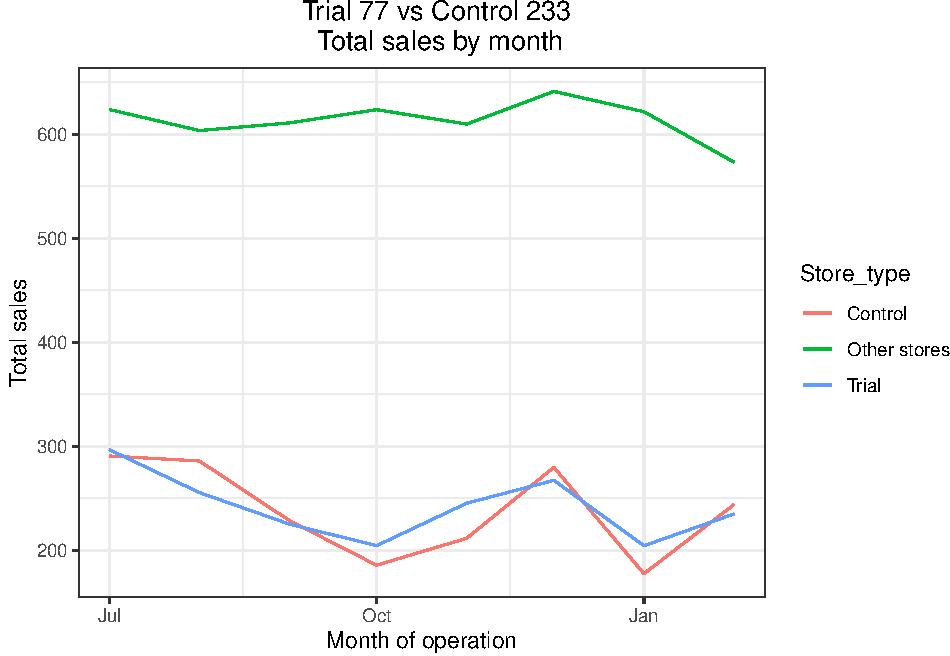
\includegraphics{Task2_files/figure-latex/unnamed-chunk-1-1}

Next, number of customers.

\begin{Shaded}
\begin{Highlighting}[]
\CommentTok{#### Over to you! Conduct visual checks on customer count trends by comparing the trial store to the control store and other stores.}
\CommentTok{#### Hint: Look at the previous plot.}

\CommentTok{# measureOverTimeCusts <- copy(measureOverTime)}
\CommentTok{# pastCustomers <- measureOverTimeCusts[, Store_type := ifelse(STORE_NBR == trial_store, "Trial",}
\CommentTok{#                                                              ifelse(STORE_NBR == control_store, }
\CommentTok{#                                                                     "Control", "Other stores"))}
\CommentTok{#                                       ][, nCustomers := mean(nCustomers) , by = c('YEARMONTH', 'Store_type')}
\CommentTok{#                                         ][, TransactionMonth := as.Date(paste(YEARMONTH %/% 100,}
\CommentTok{#                                                                               YEARMONTH %% 100, 1, }
\CommentTok{#                                                                               sep = '-'), "%Y-%m-%d")}
\CommentTok{#                                           ][YEARMONTH < 201903, ]}

\NormalTok{pastCustomers <-}\StringTok{ }\NormalTok{measureOverTime }\OperatorTok
\StringTok{  }\KeywordTok{mutate}\NormalTok{(}\DataTypeTok{Store_type =} \KeywordTok{ifelse}\NormalTok{(STORE_NBR }\OperatorTok{==}\StringTok{ }\NormalTok{trial_store, }\StringTok{"Trial"}\NormalTok{,}
                             \KeywordTok{ifelse}\NormalTok{(STORE_NBR }\OperatorTok{==}\StringTok{ }\NormalTok{control_store,}
                                    \StringTok{"Control"}\NormalTok{, }\StringTok{"Other stores"}\NormalTok{))) }\OperatorTok
\StringTok{  }\KeywordTok{group_by}\NormalTok{(YEARMONTH, Store_type) }\OperatorTok
\StringTok{  }\KeywordTok{summarise}\NormalTok{(}\DataTypeTok{nCustomers =} \KeywordTok{mean}\NormalTok{(nCustomers), }\DataTypeTok{.groups=}\StringTok{'drop'}\NormalTok{) }\OperatorTok
\StringTok{  }\KeywordTok{mutate}\NormalTok{(}\DataTypeTok{TransactionMonth =} \KeywordTok{as.Date}\NormalTok{(}\KeywordTok{paste}\NormalTok{(YEARMONTH }\OperatorTok\StringTok{ }\DecValTok{100}\NormalTok{,}
\NormalTok{                                          YEARMONTH }\OperatorTok\StringTok{ }\DecValTok{100}\NormalTok{, }\DecValTok{1}\NormalTok{,}
                                          \DataTypeTok{sep =} \StringTok{'-'}\NormalTok{)))}\OperatorTok
\StringTok{  }\KeywordTok{filter}\NormalTok{(YEARMONTH }\OperatorTok{<}\DecValTok{201903}\NormalTok{)}
\NormalTok{p2<-}\StringTok{ }\KeywordTok{ggplot}\NormalTok{(pastCustomers, }\KeywordTok{aes}\NormalTok{(TransactionMonth, nCustomers, }\DataTypeTok{color =}\NormalTok{ Store_type)) }\OperatorTok{+}
\KeywordTok{geom_line}\NormalTok{() }\OperatorTok{+}
\KeywordTok{labs}\NormalTok{(}\DataTypeTok{x =} \StringTok{'Month of operation'}\NormalTok{, }\DataTypeTok{y =} \StringTok{'Number of customers'}\NormalTok{, }
     \DataTypeTok{title =} \StringTok{"    Trial 77 vs Control 233}
\StringTok{     Total customers by month"}\NormalTok{)}
\NormalTok{p2}
\end{Highlighting}
\end{Shaded}

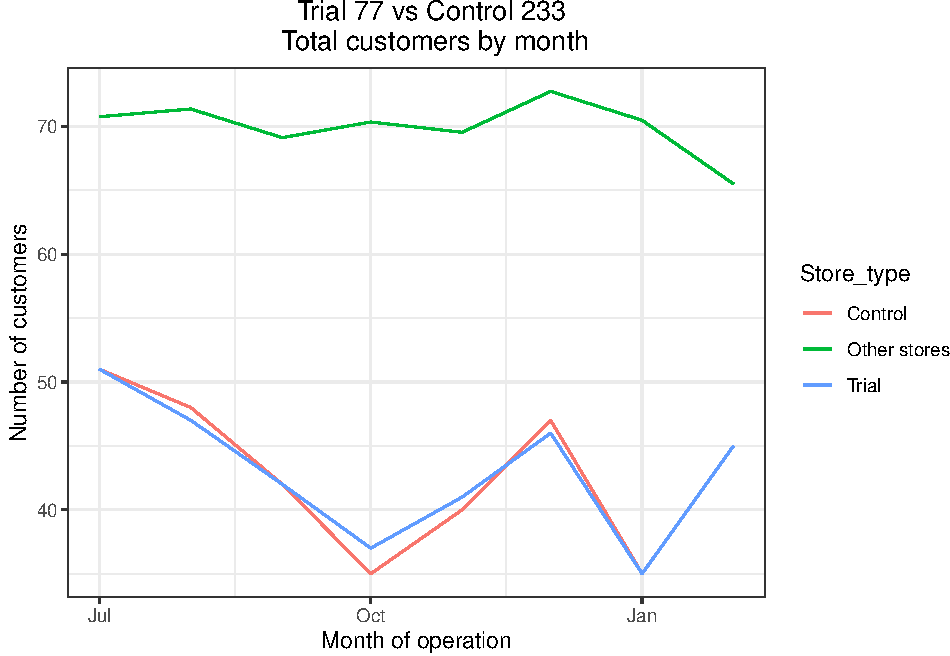
\includegraphics{Task2_files/figure-latex/unnamed-chunk-2-1}

\hypertarget{assessment-of-trial}{%
\subsection{Assessment of trial}\label{assessment-of-trial}}

The trial period goes from the start of February 2019 to April 2019. We
now want to see if there has been an uplift in overall chip sales.

We'll start with scaling the control store's sales to a level similar to
control for any differences between the two stores outside of the trial
period.

\begin{Shaded}
\begin{Highlighting}[]
\CommentTok{#### Scale pre-trial control sales to match pre-trial trial store sales}
\NormalTok{scalingFactorForControlSales <-}\StringTok{ }\NormalTok{preTrialMeasures[STORE_NBR }\OperatorTok{==}\StringTok{ }\NormalTok{trial_store }\OperatorTok{&}\StringTok{ }\NormalTok{YEARMONTH }\OperatorTok{<}\StringTok{ }\DecValTok{201902}\NormalTok{,}
                                                 \KeywordTok{sum}\NormalTok{(totSales)]}\OperatorTok{/}
\StringTok{                                }\NormalTok{preTrialMeasures[STORE_NBR }\OperatorTok{==}\StringTok{ }\NormalTok{control_store }\OperatorTok{&}\StringTok{ }\NormalTok{YEARMONTH }\OperatorTok{<}\StringTok{ }\DecValTok{201902}\NormalTok{,}
                                                 \KeywordTok{sum}\NormalTok{(totSales)]}
\CommentTok{#### Apply the scaling factor}
\NormalTok{measureOverTimeSales <-}\StringTok{ }\NormalTok{measureOverTime}
\NormalTok{scaledControlSales <-}\StringTok{ }\NormalTok{measureOverTimeSales[STORE_NBR }\OperatorTok{==}\StringTok{ }\NormalTok{control_store, }
\NormalTok{                                           ][ , controlSales }\OperatorTok{:}\ErrorTok{=}\StringTok{ }\NormalTok{totSales }\OperatorTok{*}
\StringTok{                                                }\NormalTok{scalingFactorForControlSales]}
\end{Highlighting}
\end{Shaded}

Now that we have comparable sales figures for the control store, we can
calculate the percentage difference between the scaled control sales and
the trial store's sales during the trial period.

\begin{Shaded}
\begin{Highlighting}[]
\CommentTok{#### Over to you! Calculate the percentage difference between scaled control sales and trial sales}
\NormalTok{percentageDiff <-}\StringTok{ }\KeywordTok{merge}\NormalTok{(scaledControlSales, measureOverTimeSales[STORE_NBR }\OperatorTok{==}\StringTok{ }\NormalTok{trial_store], }
                        \DataTypeTok{by =} \StringTok{'YEARMONTH'}\NormalTok{)[, percentageDiff }\OperatorTok{:}\ErrorTok{=}\StringTok{ }\KeywordTok{abs}\NormalTok{(totSales.y}\OperatorTok{/}\NormalTok{controlSales}\DecValTok{-1}\NormalTok{)]}
\end{Highlighting}
\end{Shaded}

Let's see if the difference is significant!

\begin{Shaded}
\begin{Highlighting}[]
\CommentTok{#### As our null hypothesis is that the trial period is the same as the pre-trial period, let's take the standard deviation based on the scaled percentage difference in the pre-trial period}
\NormalTok{stdDev <-}\StringTok{ }\KeywordTok{sd}\NormalTok{(percentageDiff[YEARMONTH }\OperatorTok{<}\StringTok{ }\DecValTok{201902}\NormalTok{ , percentageDiff])}
\CommentTok{#### Note that there are 8 months in the pre-trial period}
\CommentTok{#### hence 8 - 1 = 7 degrees of freedom}
\NormalTok{degreesOfFreedom <-}\StringTok{ }\DecValTok{7}
\CommentTok{#### We will test with a null hypothesis of there being 0 difference between trial and control stores.}
\CommentTok{#### Over to you! Calculate the t-values for the trial months. After that, find the 95th percentile of the t distribution with the appropriate degrees of freedom to check whether the hypothesis is statistically significant.}
\CommentTok{#### Hint: The test statistic here is (x - u)/standard deviation}
\NormalTok{percentageDiff[, tValue }\OperatorTok{:}\ErrorTok{=}\StringTok{ }\NormalTok{(percentageDiff}\DecValTok{-0}\NormalTok{)}\OperatorTok{/}\NormalTok{stdDev}
\NormalTok{               ][, TransactionMonth }\OperatorTok{:}\ErrorTok{=}\StringTok{ }\KeywordTok{as.Date}\NormalTok{(}\KeywordTok{paste}\NormalTok{(YEARMONTH }\OperatorTok\StringTok{ }\DecValTok{100}\NormalTok{,}
\NormalTok{                                          YEARMONTH }\OperatorTok\StringTok{ }\DecValTok{100}\NormalTok{, }\DecValTok{1}\NormalTok{,}
                                          \DataTypeTok{sep =} \StringTok{'-'}\NormalTok{))}
\NormalTok{                   ][, .(TransactionMonth, }
                       \DataTypeTok{percentile_95th =} \KeywordTok{qt}\NormalTok{(}\DataTypeTok{p=}\FloatTok{0.025}\NormalTok{, degreesOfFreedom, }\DataTypeTok{lower.tail =}\NormalTok{ F), }
\NormalTok{                       tValue)]}
\end{Highlighting}
\end{Shaded}

\begin{verbatim}
##     TransactionMonth percentile_95th      tValue
##  1:       2018-07-01        2.364624  0.05151525
##  2:       2018-08-01        2.364624  2.54201108
##  3:       2018-09-01        2.364624  0.75293959
##  4:       2018-10-01        2.364624  1.51840583
##  5:       2018-11-01        2.364624  2.65345950
##  6:       2018-12-01        2.364624  1.33591090
##  7:       2019-01-01        2.364624  2.50257081
##  8:       2019-02-01        2.364624  1.18353440
##  9:       2019-03-01        2.364624  7.33911567
## 10:       2019-04-01        2.364624 12.47637325
## 11:       2019-05-01        2.364624  3.02365009
## 12:       2019-06-01        2.364624  3.40609300
\end{verbatim}

We can observe that the t-value is much larger than the 95th percentile
value of the t-distribution for March and April - i.e.~the increase in
sales in the trial store in March and April is statistically greater
than in the control store.

Let's create a more visual version of this by plotting the sales of the
control store, the sales of the trial stores and the 95th percentile
value of sales of the control store.

\begin{Shaded}
\begin{Highlighting}[]
\CommentTok{# measureOverTimeSales <- copy(measureOverTime)}

\CommentTok{#### Trial and control store total sales}
\CommentTok{#### Over to you! Create new variables Store_type, totSales and TransactionMonth in the data table.}

\CommentTok{# pastSales <- measureOverTimeSales[, Store_type := ifelse(STORE_NBR==control_store, 'Control',}
\CommentTok{#                                                          ifelse(STORE_NBR==trial_store,}
\CommentTok{#                                                                 'Trial', 'Other stores'))}
\CommentTok{#                                   ][, totSales := mean(totSales),}
\CommentTok{#                                     by = c('YEARMONTH', 'Store_type')}
\CommentTok{#                                     ][, TransactionMonth := as.Date(paste(YEARMONTH %/% 100,}
\CommentTok{#                                                                           YEARMONTH %% 100, 1,}
\CommentTok{#                                                                           sep = '-'))}
\CommentTok{#                                       ][Store_type %in% c("Trial", "Control"), ]}

\NormalTok{pastSales <-}\StringTok{ }\NormalTok{measureOverTime }\OperatorTok
\StringTok{  }\KeywordTok{mutate}\NormalTok{(}\DataTypeTok{Store_type =} \KeywordTok{ifelse}\NormalTok{(STORE_NBR}\OperatorTok{==}\NormalTok{control_store, }\StringTok{'Control'}\NormalTok{,}
                             \KeywordTok{ifelse}\NormalTok{(STORE_NBR}\OperatorTok{==}\NormalTok{trial_store,}
                                    \StringTok{'Trial'}\NormalTok{, }\StringTok{'Other stores'}\NormalTok{))) }\OperatorTok
\StringTok{  }\KeywordTok{group_by}\NormalTok{(YEARMONTH, Store_type) }\OperatorTok
\StringTok{  }\KeywordTok{summarise}\NormalTok{(}\DataTypeTok{totSales =} \KeywordTok{mean}\NormalTok{(totSales), }\DataTypeTok{.groups=}\StringTok{'drop'}\NormalTok{) }\OperatorTok
\StringTok{  }\KeywordTok{mutate}\NormalTok{(}\DataTypeTok{TransactionMonth =} \KeywordTok{as.Date}\NormalTok{(}\KeywordTok{paste}\NormalTok{(YEARMONTH }\OperatorTok\StringTok{ }\DecValTok{100}\NormalTok{,}
\NormalTok{                                          YEARMONTH }\OperatorTok\StringTok{ }\DecValTok{100}\NormalTok{, }\DecValTok{1}\NormalTok{,}
                                          \DataTypeTok{sep =} \StringTok{'-'}\NormalTok{))) }\OperatorTok
\StringTok{  }\KeywordTok{filter}\NormalTok{(Store_type }\OperatorTok\StringTok{ }\KeywordTok{c}\NormalTok{(}\StringTok{'Control'}\NormalTok{, }\StringTok{'Trial'}\NormalTok{))}


\CommentTok{#### Control store 95th percentile}
\NormalTok{pastSales_Controls95 <-}\StringTok{ }\NormalTok{pastSales}\OperatorTok
\StringTok{  }\KeywordTok{filter}\NormalTok{(Store_type }\OperatorTok{==}\StringTok{ 'Control'}\NormalTok{) }\OperatorTok
\StringTok{  }\KeywordTok{mutate}\NormalTok{(}\DataTypeTok{totSales =}\NormalTok{ totSales }\OperatorTok{*}\NormalTok{(}\DecValTok{1}\OperatorTok{+}\NormalTok{stdDev}\OperatorTok{*}\DecValTok{2}\NormalTok{),}
         \DataTypeTok{Store_type =} \StringTok{'Control 95th % confidence interval'}\NormalTok{)}
\CommentTok{# pastSales_Controls95 <- pastSales[Store_type == "Control",}
\CommentTok{#                                   ][, totSales := totSales + (stdDev * 2)}
\CommentTok{#                                     ][, Store_type := "Control 95th % confidence interval"]}
\CommentTok{#### Control store 5th percentile}
\NormalTok{pastSales_Controls5 <-}\StringTok{ }\NormalTok{pastSales}\OperatorTok
\StringTok{  }\KeywordTok{filter}\NormalTok{(Store_type }\OperatorTok{==}\StringTok{ 'Control'}\NormalTok{) }\OperatorTok
\StringTok{  }\KeywordTok{mutate}\NormalTok{(}\DataTypeTok{totSales =}\NormalTok{ totSales }\OperatorTok{*}\NormalTok{(}\DecValTok{1}\OperatorTok{-}\NormalTok{stdDev}\OperatorTok{*}\DecValTok{2}\NormalTok{),}
         \DataTypeTok{Store_type =} \StringTok{'Control 5th % confidence interval'}\NormalTok{)}
\CommentTok{# pastSales_Controls5 <- pastSales[Store_type == "Control",}
\CommentTok{#                                  ][, totSales := totSales - (stdDev * 2)}
\CommentTok{#                                    ][, Store_type := "Control 5th % confidence interval"]}
\NormalTok{trialAssessment <-}\StringTok{ }\KeywordTok{rbind}\NormalTok{(pastSales, pastSales_Controls95, pastSales_Controls5)}
\CommentTok{#### Plotting these in one nice graph}
\NormalTok{pp1 <-}\StringTok{ }\KeywordTok{ggplot}\NormalTok{(trialAssessment, }\KeywordTok{aes}\NormalTok{(TransactionMonth, totSales, }\DataTypeTok{color =}\NormalTok{ Store_type)) }\OperatorTok{+}
\KeywordTok{geom_rect}\NormalTok{(}\DataTypeTok{data =}\NormalTok{ trialAssessment }\OperatorTok\StringTok{ }\KeywordTok{filter}\NormalTok{(YEARMONTH }\OperatorTok{<}\StringTok{ }\DecValTok{201905} \OperatorTok{&}\StringTok{ }\NormalTok{YEARMONTH }\OperatorTok{>}\StringTok{ }\DecValTok{201901}\NormalTok{) ,}
\KeywordTok{aes}\NormalTok{(}\DataTypeTok{xmin =} \KeywordTok{min}\NormalTok{(TransactionMonth), }\DataTypeTok{xmax =} \KeywordTok{max}\NormalTok{(TransactionMonth), }\DataTypeTok{ymin =} \DecValTok{0}\NormalTok{ , }\DataTypeTok{ymax =}
\OtherTok{Inf}\NormalTok{, }\DataTypeTok{color =} \OtherTok{NULL}\NormalTok{), }\DataTypeTok{show.legend =} \OtherTok{FALSE}\NormalTok{) }\OperatorTok{+}
\KeywordTok{geom_line}\NormalTok{() }\OperatorTok{+}
\KeywordTok{labs}\NormalTok{(}\DataTypeTok{x =} \StringTok{"Month of operation"}\NormalTok{, }\DataTypeTok{y =} \StringTok{"Total sales"}\NormalTok{, }
     \DataTypeTok{title =} \StringTok{"Total sales by month  - Trial 77 Control 233"}\NormalTok{)}
\NormalTok{pp1}
\end{Highlighting}
\end{Shaded}

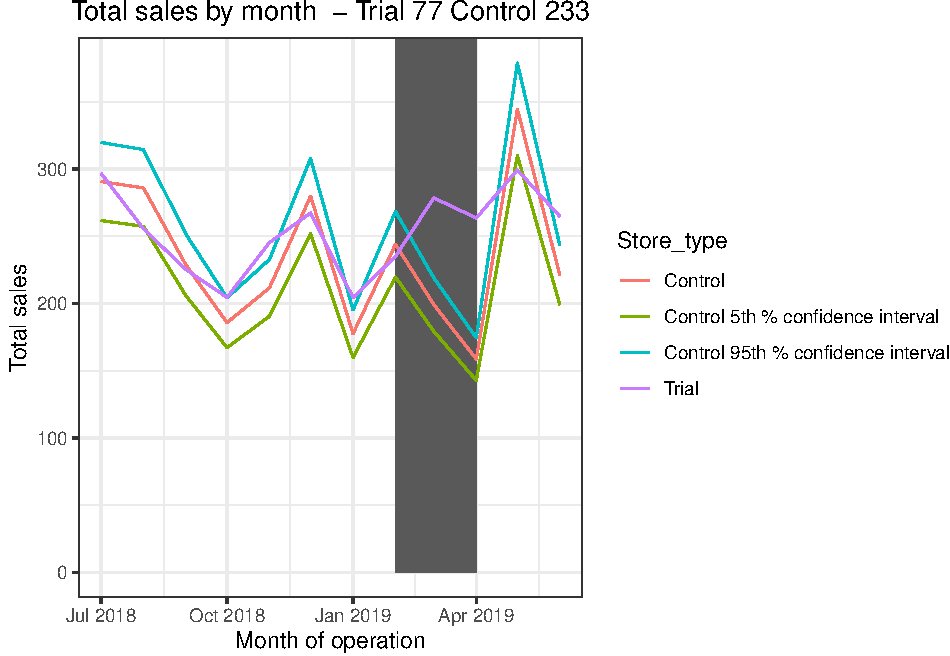
\includegraphics{Task2_files/figure-latex/unnamed-chunk-5-1}

Let's have a look at assessing this for number of customers as well.

\begin{Shaded}
\begin{Highlighting}[]
\CommentTok{#### This would be a repeat of the steps before for total sales}
\CommentTok{#### Scale pre-trial control customers to match pre-trial trial store customers}
\CommentTok{#### Over to you! Compute a scaling factor to align control store customer counts to our trial store.}
\CommentTok{#### Then, apply the scaling factor to control store customer counts.}
\CommentTok{#### Finally, calculate the percentage difference between scaled control store customers and trial customers.}

\NormalTok{scalingFactorForControlCust <-}\StringTok{ }\NormalTok{preTrialMeasures[STORE_NBR}\OperatorTok{==}\NormalTok{trial_store, }\KeywordTok{sum}\NormalTok{(nCustomers)]}\OperatorTok{/}
\StringTok{                               }\NormalTok{preTrialMeasures[STORE_NBR}\OperatorTok{==}\NormalTok{control_store, }\KeywordTok{sum}\NormalTok{(nCustomers)]}
\NormalTok{measureOverTimeCusts <-}\StringTok{ }\NormalTok{measureOverTime}
\NormalTok{scaledControlCustomers <-}\StringTok{ }\NormalTok{measureOverTimeCusts[STORE_NBR}\OperatorTok{==}\NormalTok{control_store,}
\NormalTok{                                               ][, controlCustomers }\OperatorTok{:}\ErrorTok{=}\StringTok{ }\NormalTok{nCustomers}\OperatorTok{*}\NormalTok{scalingFactorForControlCust}
\NormalTok{                                                 ][, Store_type }\OperatorTok{:}\ErrorTok{=}\StringTok{ 'Control'}\NormalTok{]}
\NormalTok{percentageDiff <-}\StringTok{ }\KeywordTok{merge}\NormalTok{(scaledControlCustomers, measureOverTimeCusts[STORE_NBR}\OperatorTok{==}\NormalTok{trial_store,],}
                        \DataTypeTok{by =} \StringTok{'YEARMONTH'}\NormalTok{)[, percentageDiff}\OperatorTok{:}\ErrorTok{=}\StringTok{ }\KeywordTok{abs}\NormalTok{(nCustomers.y}\OperatorTok{/}\NormalTok{controlCustomers}\DecValTok{-1}\NormalTok{)]}
\end{Highlighting}
\end{Shaded}

Let's again see if the difference is significant visually!

\begin{Shaded}
\begin{Highlighting}[]
\CommentTok{#### As our null hypothesis is that the trial period is the same as the pre-trial period, let's take the standard deviation based on the scaled percentage difference in the pre-trial period}
\NormalTok{stdDev <-}\StringTok{ }\KeywordTok{sd}\NormalTok{(percentageDiff[YEARMONTH }\OperatorTok{<}\StringTok{ }\DecValTok{201902}\NormalTok{ , percentageDiff])}
\NormalTok{degreesOfFreedom <-}\StringTok{ }\DecValTok{7}
\CommentTok{# percentageDiff[, tValue:= (percentageDiff-0)/stdDev}
\CommentTok{#                ][, TransactionMonth := as.Date(paste(YEARMONTH %/% 100,}
\CommentTok{#                                                      YEARMONTH %% 100, 1,}
\CommentTok{#                                                      sep='-'), format = '%Y-%m-%d')}
\CommentTok{#                  ][, .(TransactionMonth, }
\CommentTok{#                        percentile_95th = qt(p=0.025, degreesOfFreedom, lower.tail = F), }
\CommentTok{#                        tValue)]}
\CommentTok{#### Trial and control store number of customers}
\NormalTok{pastCustomers <-}\StringTok{ }\NormalTok{measureOverTimeCusts[, Store_type}\OperatorTok{:}\ErrorTok{=}\StringTok{ }\KeywordTok{ifelse}\NormalTok{(STORE_NBR}\OperatorTok{==}\NormalTok{control_store, }\StringTok{'Control'}\NormalTok{,}
                                                            \KeywordTok{ifelse}\NormalTok{(STORE_NBR}\OperatorTok{==}\NormalTok{trial_store, }\StringTok{'Trial'}\NormalTok{,}
                                                                   \StringTok{'Other stores'}\NormalTok{))}
\NormalTok{                                      ][, nCusts }\OperatorTok{:}\ErrorTok{=}\StringTok{ }\KeywordTok{mean}\NormalTok{(nCustomers), }
\NormalTok{                                        by =}\StringTok{ }\KeywordTok{c}\NormalTok{(}\StringTok{"YEARMONTH"}\NormalTok{, }\StringTok{"Store_type"}\NormalTok{)}
\NormalTok{                                      ][, TransactionMonth }\OperatorTok{:}\ErrorTok{=}\StringTok{ }\KeywordTok{as.Date}\NormalTok{(}\KeywordTok{paste}\NormalTok{(YEARMONTH }\OperatorTok\DecValTok{100}\NormalTok{,}
\NormalTok{                                                                            YEARMONTH }\OperatorTok\StringTok{ }\DecValTok{100}\NormalTok{, }\DecValTok{1}\NormalTok{,}
                                                                            \DataTypeTok{sep=}\StringTok{'-'}\NormalTok{),}
                                                                      \DataTypeTok{format =} \StringTok{'%Y-%m-%d'}\NormalTok{)}
\NormalTok{                                        ][Store_type }\OperatorTok\StringTok{ }\KeywordTok{c}\NormalTok{(}\StringTok{"Trial"}\NormalTok{, }\StringTok{"Control"}\NormalTok{), ]}
\CommentTok{#### Control store 95th percentile}
\NormalTok{pastCustomers_Controls95 <-}\StringTok{ }\NormalTok{pastCustomers[Store_type }\OperatorTok{==}\StringTok{ "Control"}\NormalTok{,}
\NormalTok{                                          ][, nCusts }\OperatorTok{:}\ErrorTok{=}\StringTok{ }\NormalTok{nCusts }\OperatorTok{*}\StringTok{ }\NormalTok{(}\DecValTok{1} \OperatorTok{+}\StringTok{ }\NormalTok{stdDev }\OperatorTok{*}\StringTok{ }\DecValTok{2}\NormalTok{)}
\NormalTok{                                          ][, Store_type }\OperatorTok{:}\ErrorTok{=}\StringTok{ "Control 95th % confidence interval"}\NormalTok{]}
\CommentTok{#### Control store 5th percentile}
\NormalTok{pastCustomers_Controls5 <-}\StringTok{ }\NormalTok{pastCustomers[Store_type }\OperatorTok{==}\StringTok{ "Control"}\NormalTok{,}
\NormalTok{                                         ][, nCusts }\OperatorTok{:}\ErrorTok{=}\StringTok{ }\NormalTok{nCusts }\OperatorTok{*}\StringTok{ }\NormalTok{(}\DecValTok{1} \OperatorTok{-}\StringTok{ }\NormalTok{stdDev }\OperatorTok{*}\StringTok{ }\DecValTok{2}\NormalTok{)}
\NormalTok{                                         ][, Store_type }\OperatorTok{:}\ErrorTok{=}\StringTok{ "Control 5th % confidence interval"}\NormalTok{]}
\NormalTok{trialAssessment <-}\StringTok{ }\KeywordTok{rbind}\NormalTok{(pastCustomers, }
\NormalTok{                         pastCustomers_Controls95,}
\NormalTok{                         pastCustomers_Controls5)}
\CommentTok{#### Over to you! Plot everything into one nice graph.}
\CommentTok{#### Hint: geom_rect creates a rectangle in the plot. Use this to highlight the trial period in our graph.}
\NormalTok{pp2 <-}\StringTok{ }\KeywordTok{ggplot}\NormalTok{(trialAssessment, }\KeywordTok{aes}\NormalTok{(TransactionMonth, nCusts, }\DataTypeTok{color=}\NormalTok{Store_type)) }\OperatorTok{+}
\KeywordTok{geom_rect}\NormalTok{(}\DataTypeTok{data =}\NormalTok{ trialAssessment[YEARMONTH}\OperatorTok{<}\DecValTok{201905}\OperatorTok{&}\NormalTok{YEARMONTH}\OperatorTok{>}\DecValTok{201901}\NormalTok{,], }
          \KeywordTok{aes}\NormalTok{(}\DataTypeTok{xmin =} \KeywordTok{min}\NormalTok{(TransactionMonth), }\DataTypeTok{xmax =} \KeywordTok{max}\NormalTok{(TransactionMonth), }
              \DataTypeTok{ymin =} \DecValTok{0}\NormalTok{, }\DataTypeTok{ymax =} \OtherTok{Inf}\NormalTok{, }\DataTypeTok{color =} \OtherTok{NULL}\NormalTok{), }\DataTypeTok{show.legend =} \OtherTok{FALSE}\NormalTok{) }\OperatorTok{+}
\KeywordTok{geom_line}\NormalTok{() }\OperatorTok{+}
\KeywordTok{labs}\NormalTok{(}\DataTypeTok{x =} \StringTok{'Month of operation'}\NormalTok{, }\DataTypeTok{y =} \StringTok{'Total customer'}\NormalTok{, }
     \DataTypeTok{title =} \StringTok{'Total customer by months - Trial 77 Control 233'}\NormalTok{)}
\NormalTok{pp2}
\end{Highlighting}
\end{Shaded}

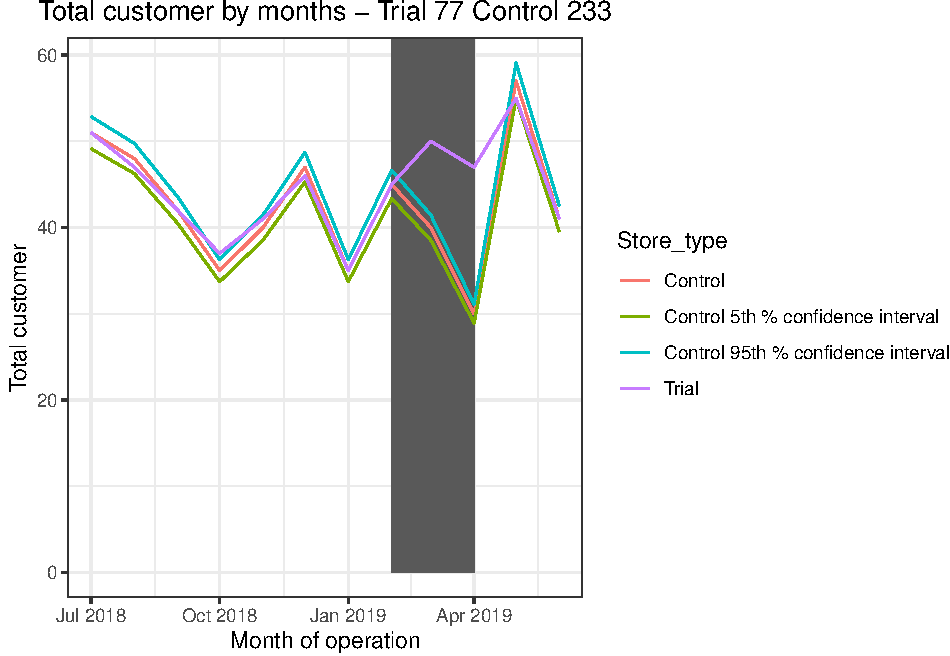
\includegraphics{Task2_files/figure-latex/unnamed-chunk-7-1}

Let's repeat finding the control store and assessing the impact of the
trial for each of the other two trial stores.

\hypertarget{trial-store-86}{%
\subsection{Trial store 86}\label{trial-store-86}}

\begin{Shaded}
\begin{Highlighting}[]
\CommentTok{#### Over to you! Calculate the metrics below as we did for the first trial store.}
\NormalTok{measureOverTime <-}\StringTok{ }\NormalTok{data[, .(}\DataTypeTok{totSales =} \KeywordTok{sum}\NormalTok{(TOT_SALES),}
                            \DataTypeTok{nCustomers =} \KeywordTok{uniqueN}\NormalTok{(LYLTY_CARD_NBR),}
                            \DataTypeTok{nTxnPerCust =} \KeywordTok{uniqueN}\NormalTok{(TXN_ID)}\OperatorTok{/}\KeywordTok{uniqueN}\NormalTok{(LYLTY_CARD_NBR),}
                            \DataTypeTok{nChipsPerTxn =} \KeywordTok{sum}\NormalTok{(PROD_QTY)}\OperatorTok{/}\KeywordTok{uniqueN}\NormalTok{(TXN_ID),}
                            \DataTypeTok{avgPricePerUnit =} \KeywordTok{sum}\NormalTok{(TOT_SALES)}\OperatorTok{/}\KeywordTok{sum}\NormalTok{(PROD_QTY)}
\NormalTok{                            ), by =}\StringTok{ }\NormalTok{.(STORE_NBR, YEARMONTH)][}\KeywordTok{order}\NormalTok{(STORE_NBR,YEARMONTH)]}

\NormalTok{storesWithFullObs <-}\StringTok{ }\KeywordTok{unique}\NormalTok{(measureOverTime[, .N, STORE_NBR][N }\OperatorTok{==}\StringTok{ }\DecValTok{12}\NormalTok{, STORE_NBR])}
\NormalTok{preTrialMeasures <-}\StringTok{ }\NormalTok{measureOverTime[YEARMONTH }\OperatorTok{<}\StringTok{ }\DecValTok{201902} \OperatorTok{&}\StringTok{ }\NormalTok{STORE_NBR }\OperatorTok\StringTok{ }\NormalTok{storesWithFullObs, ]}
\CommentTok{#### Over to you! Use the functions we created earlier to calculate correlation and magnitude for each potential control store}
\NormalTok{trial_store <-}\StringTok{ }\DecValTok{86}
\NormalTok{corr_nSales <-}\StringTok{ }\KeywordTok{calculateCorrelation}\NormalTok{(preTrialMeasures, }\KeywordTok{quote}\NormalTok{(totSales), trial_store)}
\NormalTok{corr_nCustomers <-}\StringTok{ }\KeywordTok{calculateCorrelation}\NormalTok{(preTrialMeasures, }\KeywordTok{quote}\NormalTok{(nCustomers), trial_store)}
\NormalTok{magnitude_nSales <-}\StringTok{ }\KeywordTok{calculateMagnitudeDistance}\NormalTok{(preTrialMeasures, }\KeywordTok{quote}\NormalTok{(totSales), trial_store)}
\NormalTok{magnitude_nCustomers <-}\StringTok{ }\KeywordTok{calculateMagnitudeDistance}\NormalTok{(preTrialMeasures, }\KeywordTok{quote}\NormalTok{(nCustomers), trial_store)}

\CommentTok{#### Now, create a combined score composed of correlation and magnitude}
\NormalTok{corr_weight <-}\StringTok{ }\FloatTok{0.5}
\NormalTok{score_nSales <-}\StringTok{ }\KeywordTok{merge}\NormalTok{(corr_nSales, magnitude_nSales, }
                      \DataTypeTok{by =} \KeywordTok{c}\NormalTok{(}\StringTok{'Store1'}\NormalTok{,}\StringTok{'Store2'}\NormalTok{)}
\NormalTok{                      )[, scoreNSales }\OperatorTok{:}\ErrorTok{=}\StringTok{ }\NormalTok{corr_weight}\OperatorTok{*}\NormalTok{corr_measure}\OperatorTok{+}\NormalTok{(}\DecValTok{1}\OperatorTok{-}\NormalTok{corr_weight)}\OperatorTok{*}\NormalTok{mag_measure]}
\NormalTok{score_nCustomers <-}\StringTok{ }\KeywordTok{merge}\NormalTok{(corr_nCustomers, magnitude_nCustomers, }
                      \DataTypeTok{by =} \KeywordTok{c}\NormalTok{(}\StringTok{'Store1'}\NormalTok{,}\StringTok{'Store2'}\NormalTok{)}
\NormalTok{                      )[, scoreNCust }\OperatorTok{:}\ErrorTok{=}\StringTok{ }\NormalTok{corr_weight}\OperatorTok{*}\NormalTok{corr_measure}\OperatorTok{+}\NormalTok{(}\DecValTok{1}\OperatorTok{-}\NormalTok{corr_weight)}\OperatorTok{*}\NormalTok{mag_measure]}
\CommentTok{#### Finally, combine scores across the drivers using a simple average.}
\NormalTok{score_Control <-}\StringTok{ }\KeywordTok{merge}\NormalTok{(score_nSales, score_nCustomers, }\DataTypeTok{by =} \KeywordTok{c}\NormalTok{(}\StringTok{'Store1'}\NormalTok{,}\StringTok{'Store2'}\NormalTok{))}
\NormalTok{score_Control[, finalControlScore }\OperatorTok{:}\ErrorTok{=}\StringTok{ }\NormalTok{(scoreNSales}\OperatorTok{+}\NormalTok{scoreNCust)}\OperatorTok{/}\DecValTok{2}\NormalTok{]}
\CommentTok{#### Select control stores based on the highest matching store}
\CommentTok{#### (closest to 1 but not the store itself, i.e. the second ranked highest store)}
\CommentTok{#### Select control store for trial store 86}
\NormalTok{control_store <-}\StringTok{ }\NormalTok{score_Control[Store1 }\OperatorTok{==}\StringTok{ }\NormalTok{trial_store,}
\NormalTok{                               ][}\KeywordTok{order}\NormalTok{(}\OperatorTok{-}\NormalTok{finalControlScore)][}\DecValTok{2}\NormalTok{, Store2]}
\NormalTok{control_store}
\end{Highlighting}
\end{Shaded}

\begin{verbatim}
## [1] 155
\end{verbatim}

Looks like store 155 will be a control store for trial store 86.

Again, let's check visually if the drivers are indeed similar in the
period before the trial.

We'll look at total sales first.

\begin{Shaded}
\begin{Highlighting}[]
\CommentTok{#### Over to you! Conduct visual checks on trends based on the drivers}

\NormalTok{pastSales <-}\StringTok{ }\NormalTok{measureOverTime }\OperatorTok
\StringTok{  }\KeywordTok{mutate}\NormalTok{(}\DataTypeTok{Store_type =} \KeywordTok{ifelse}\NormalTok{(STORE_NBR}\OperatorTok{==}\NormalTok{control_store, }\StringTok{'Control'}\NormalTok{,}
                             \KeywordTok{ifelse}\NormalTok{(STORE_NBR}\OperatorTok{==}\NormalTok{trial_store,}\StringTok{'Trial'}\NormalTok{,}
                                    \StringTok{'Other stores'}\NormalTok{))) }\OperatorTok
\StringTok{  }\KeywordTok{group_by}\NormalTok{(YEARMONTH, Store_type) }\OperatorTok
\StringTok{  }\KeywordTok{summarise}\NormalTok{(}\DataTypeTok{totSales =} \KeywordTok{mean}\NormalTok{(totSales), }\DataTypeTok{.groups =} \StringTok{'drop'}\NormalTok{) }\OperatorTok
\StringTok{  }\KeywordTok{mutate}\NormalTok{(}\DataTypeTok{TransactionMonth =} \KeywordTok{as.Date}\NormalTok{(}\KeywordTok{paste}\NormalTok{(YEARMONTH }\OperatorTok\StringTok{ }\DecValTok{100}\NormalTok{,}
\NormalTok{                                          YEARMONTH }\OperatorTok\StringTok{ }\DecValTok{100}\NormalTok{, }\DecValTok{1}\NormalTok{,}
                                          \DataTypeTok{sep=}\StringTok{'-'}\NormalTok{), }\DataTypeTok{format =} \StringTok{'%Y-%m-%d'}\NormalTok{)) }\OperatorTok
\StringTok{  }\KeywordTok{filter}\NormalTok{(YEARMONTH}\OperatorTok{<}\DecValTok{201903}\NormalTok{)}

\NormalTok{p3<-}\KeywordTok{ggplot}\NormalTok{(pastSales, }\KeywordTok{aes}\NormalTok{(TransactionMonth, totSales, }\DataTypeTok{color =}\NormalTok{ Store_type)) }\OperatorTok{+}
\KeywordTok{geom_line}\NormalTok{() }\OperatorTok{+}
\KeywordTok{labs}\NormalTok{(}\DataTypeTok{x=}\StringTok{'Month of operation'}\NormalTok{, }\DataTypeTok{y=}\StringTok{'Total sales'}\NormalTok{, }
     \DataTypeTok{title =} \StringTok{'    Trial 86 vs Control 155}
\StringTok{     Total sales by month'}\NormalTok{)}
\NormalTok{p3}
\end{Highlighting}
\end{Shaded}

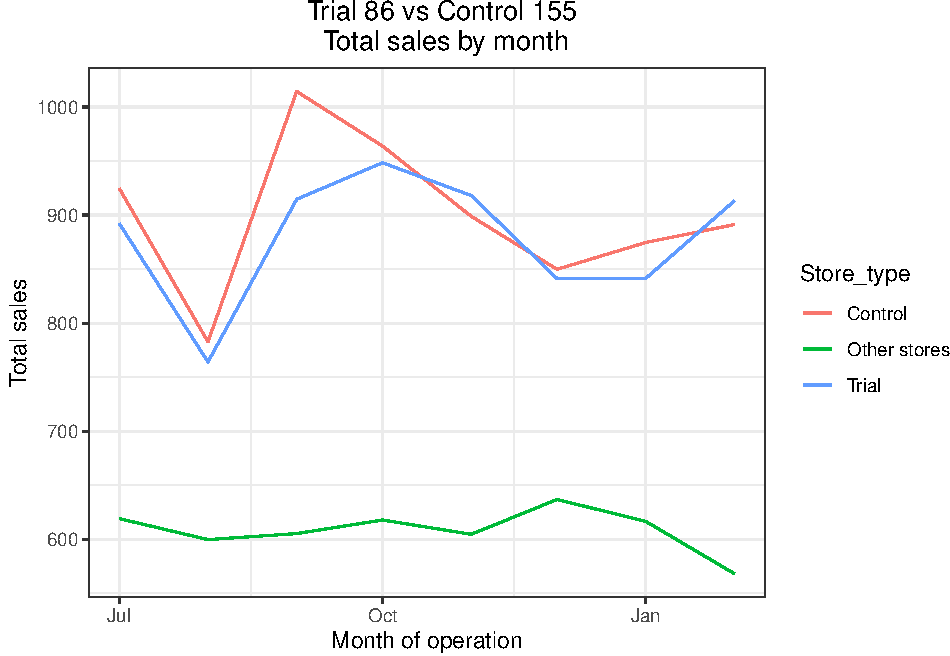
\includegraphics{Task2_files/figure-latex/unnamed-chunk-9-1.pdf} Great,
sales are trending in a similar way. Next, number of customers.

\begin{Shaded}
\begin{Highlighting}[]
\CommentTok{#### Over to you again! Conduct visual checks on trends based on the drivers}
\NormalTok{pastCustomers <-}\StringTok{ }\NormalTok{measureOverTime }\OperatorTok
\StringTok{  }\KeywordTok{mutate}\NormalTok{(}\DataTypeTok{Store_type =} \KeywordTok{ifelse}\NormalTok{(STORE_NBR}\OperatorTok{==}\NormalTok{control_store, }\StringTok{'Control'}\NormalTok{,}
                             \KeywordTok{ifelse}\NormalTok{(STORE_NBR}\OperatorTok{==}\NormalTok{trial_store,}\StringTok{'Trial'}\NormalTok{,}
                                    \StringTok{'Other stores'}\NormalTok{))) }\OperatorTok
\StringTok{  }\KeywordTok{group_by}\NormalTok{(YEARMONTH, Store_type) }\OperatorTok
\StringTok{  }\KeywordTok{summarise}\NormalTok{(}\DataTypeTok{numberCustomers =} \KeywordTok{mean}\NormalTok{(nCustomers), }\DataTypeTok{.groups =} \StringTok{'drop'}\NormalTok{) }\OperatorTok
\StringTok{  }\KeywordTok{mutate}\NormalTok{(}\DataTypeTok{TransactionMonth =} \KeywordTok{as.Date}\NormalTok{(}\KeywordTok{paste}\NormalTok{(YEARMONTH }\OperatorTok\StringTok{ }\DecValTok{100}\NormalTok{,}
\NormalTok{                                          YEARMONTH }\OperatorTok\StringTok{ }\DecValTok{100}\NormalTok{, }\DecValTok{1}\NormalTok{,}
                                          \DataTypeTok{sep=}\StringTok{'-'}\NormalTok{), }\DataTypeTok{format =} \StringTok{'%Y-%m-%d'}\NormalTok{)) }\OperatorTok
\StringTok{  }\KeywordTok{filter}\NormalTok{(YEARMONTH }\OperatorTok{<}\DecValTok{201903}\NormalTok{)}
\NormalTok{p4<-}\KeywordTok{ggplot}\NormalTok{(pastCustomers, }\KeywordTok{aes}\NormalTok{(TransactionMonth, numberCustomers, }\DataTypeTok{color=}\NormalTok{Store_type)) }\OperatorTok{+}
\KeywordTok{geom_line}\NormalTok{() }\OperatorTok{+}
\KeywordTok{labs}\NormalTok{(}\DataTypeTok{x=}\StringTok{'Month of operation'}\NormalTok{, }\DataTypeTok{y=}\StringTok{'Number of customers'}\NormalTok{, }
     \DataTypeTok{title =} \StringTok{'    Trial 86 vs Control 155}
\StringTok{     Total customers by month'}\NormalTok{)}
\NormalTok{p4}
\end{Highlighting}
\end{Shaded}

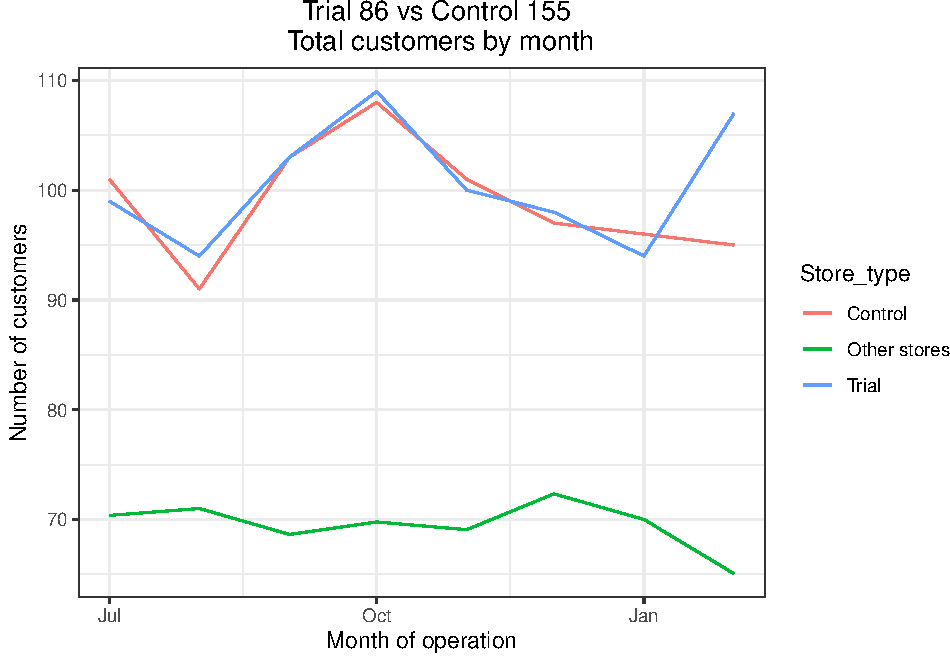
\includegraphics{Task2_files/figure-latex/unnamed-chunk-10-1.pdf}

Good, the trend in number of customers is also similar.

Let's now assess the impact of the trial on sales.

\begin{Shaded}
\begin{Highlighting}[]
\CommentTok{#### Scale pre-trial control sales to match pre-trial trial store sales}
\NormalTok{scalingFactorForControlSales <-}\StringTok{ }\NormalTok{preTrialMeasures[STORE_NBR }\OperatorTok{==}\StringTok{ }\NormalTok{trial_store, }\KeywordTok{sum}\NormalTok{(totSales)]}\OperatorTok{/}
\StringTok{                                }\NormalTok{preTrialMeasures[STORE_NBR }\OperatorTok{==}\StringTok{ }\NormalTok{control_store, }\KeywordTok{sum}\NormalTok{(totSales)]}
\CommentTok{#### Apply the scaling factor}
\NormalTok{measureOverTimeSales <-}\StringTok{ }\NormalTok{measureOverTime}
\NormalTok{scaledControlSales <-}\StringTok{ }\NormalTok{measureOverTimeSales[STORE_NBR }\OperatorTok{==}\StringTok{ }\NormalTok{control_store, }
\NormalTok{                                           ][ ,controlSales }\OperatorTok{:}\ErrorTok{=}\StringTok{ }\NormalTok{totSales }\OperatorTok{*}
\StringTok{                                                }\NormalTok{scalingFactorForControlSales]}
\CommentTok{#### Over to you! Calculate the percentage difference between scaled control sales and trial sales}
\CommentTok{#### Hint: When calculating percentage difference, remember to use absolute difference}
\NormalTok{percentageDiff <-}\StringTok{ }\KeywordTok{merge}\NormalTok{(scaledControlSales, }
\NormalTok{                        measureOverTimeSales[STORE_NBR}\OperatorTok{==}\NormalTok{trial_store,],}
                        \DataTypeTok{by =} \StringTok{"YEARMONTH"}
\NormalTok{                        )[, percentageDiff }\OperatorTok{:}\ErrorTok{=}\StringTok{ }\KeywordTok{abs}\NormalTok{(totSales.y}\OperatorTok{/}\NormalTok{controlSales}\DecValTok{-1}\NormalTok{)]}
\CommentTok{#### As our null hypothesis is that the trial period is the same as the pre-trial period, let's take the standard deviation based on the scaled percentage difference in the pre-trial period}
\CommentTok{#### Over to you! Calculate the standard deviation of percentage differences during the pre-trial period}
\NormalTok{stdDev <-}\StringTok{ }\KeywordTok{sd}\NormalTok{(percentageDiff[YEARMONTH}\OperatorTok{<}\DecValTok{201902}\NormalTok{, percentageDiff])}
\NormalTok{degreesOfFreedom <-}\StringTok{ }\DecValTok{7}
\CommentTok{#### Trial and control store total sales}
\CommentTok{#### Over to you! Create a table with sales by store type and month.}
\CommentTok{#### Hint: We only need data for the trial and control store.}

\NormalTok{pastSales <-}\StringTok{ }\NormalTok{measureOverTime }\OperatorTok
\StringTok{  }\KeywordTok{mutate}\NormalTok{(}\DataTypeTok{Store_type =} \KeywordTok{ifelse}\NormalTok{(STORE_NBR}\OperatorTok{==}\NormalTok{control_store, }\StringTok{'Control'}\NormalTok{,}
                             \KeywordTok{ifelse}\NormalTok{(STORE_NBR}\OperatorTok{==}\NormalTok{trial_store, }\StringTok{'Trial'}\NormalTok{,}
                                    \StringTok{'Other stores'}\NormalTok{))) }\OperatorTok
\StringTok{  }\KeywordTok{group_by}\NormalTok{(YEARMONTH, Store_type) }\OperatorTok
\StringTok{  }\KeywordTok{summarise}\NormalTok{(}\DataTypeTok{totSales =} \KeywordTok{mean}\NormalTok{(totSales), }\DataTypeTok{.groups =} \StringTok{'drop'}\NormalTok{) }\OperatorTok
\StringTok{  }\KeywordTok{mutate}\NormalTok{(}\DataTypeTok{TransactionMonth =} \KeywordTok{as.Date}\NormalTok{(}\KeywordTok{paste}\NormalTok{(YEARMONTH }\OperatorTok\StringTok{ }\DecValTok{100}\NormalTok{,}
\NormalTok{                                          YEARMONTH }\OperatorTok\StringTok{ }\DecValTok{100}\NormalTok{, }\DecValTok{1}\NormalTok{,}
                                          \DataTypeTok{sep =} \StringTok{'-'}\NormalTok{))) }\OperatorTok
\StringTok{  }\KeywordTok{filter}\NormalTok{(Store_type }\OperatorTok\StringTok{ }\KeywordTok{c}\NormalTok{(}\StringTok{'Control'}\NormalTok{, }\StringTok{'Trial'}\NormalTok{))}
\CommentTok{#### Over to you! Calculate the 5th and 95th percentile for control store sales.}
\CommentTok{#### Hint: The 5th and 95th percentiles can be approximated by using two standard deviations away from the mean.}
\CommentTok{#### Hint2: Recall that the variable stdDev earlier calculates standard deviation in percentages, and not dollar sales.}
\NormalTok{pastSales_Controls95 <-}\StringTok{ }\NormalTok{pastSales }\OperatorTok
\StringTok{  }\KeywordTok{filter}\NormalTok{(Store_type}\OperatorTok{==}\StringTok{'Control'}\NormalTok{) }\OperatorTok
\StringTok{  }\KeywordTok{mutate}\NormalTok{(}\DataTypeTok{totSales =}\NormalTok{ totSales}\OperatorTok{*}\NormalTok{(}\DecValTok{1}\OperatorTok{+}\StringTok{ }\NormalTok{stdDev}\OperatorTok{*}\DecValTok{2}\NormalTok{),}
         \DataTypeTok{Store_type =} \StringTok{'Control 95th % confidence interval'}\NormalTok{)}
\NormalTok{pastSales_Controls5 <-}\StringTok{  }\NormalTok{pastSales }\OperatorTok
\StringTok{  }\KeywordTok{filter}\NormalTok{(Store_type }\OperatorTok{==}\StringTok{ 'Control'}\NormalTok{) }\OperatorTok
\StringTok{  }\KeywordTok{mutate}\NormalTok{(}\DataTypeTok{totSales =}\NormalTok{ totSales}\OperatorTok{*}\NormalTok{(}\DecValTok{1} \OperatorTok{-}\StringTok{ }\NormalTok{stdDev}\OperatorTok{*}\DecValTok{2}\NormalTok{),}
         \DataTypeTok{Store_type =} \StringTok{"Control 5th % confidence interval"}\NormalTok{)}
\CommentTok{#### Then, create a combined table with columns from pastSales, pastSales_Controls95 and pastSales_Controls5}
\NormalTok{trialAssessment <-}\StringTok{ }\KeywordTok{rbind}\NormalTok{(pastSales, }
\NormalTok{                         pastSales_Controls95,}
\NormalTok{                         pastSales_Controls5)}
\CommentTok{#### Plotting these in one nice graph}
\NormalTok{pp3<-}\KeywordTok{ggplot}\NormalTok{(trialAssessment, }\KeywordTok{aes}\NormalTok{(TransactionMonth, totSales, }\DataTypeTok{color =}\NormalTok{ Store_type)) }\OperatorTok{+}
\StringTok{  }\KeywordTok{geom_rect}\NormalTok{(}\DataTypeTok{data =}\NormalTok{ trialAssessment}\OperatorTok\KeywordTok{filter}\NormalTok{(YEARMONTH }\OperatorTok{<}\StringTok{ }\DecValTok{201905} \OperatorTok{&}\StringTok{ }\NormalTok{YEARMONTH }\OperatorTok{>}\StringTok{ }\DecValTok{201901}\NormalTok{),}
            \KeywordTok{aes}\NormalTok{(}\DataTypeTok{xmin =} \KeywordTok{min}\NormalTok{(TransactionMonth), }\DataTypeTok{xmax =} \KeywordTok{max}\NormalTok{(TransactionMonth), }
                \DataTypeTok{ymin =} \DecValTok{0}\NormalTok{ , }\DataTypeTok{ymax =}\OtherTok{Inf}\NormalTok{, }\DataTypeTok{color =} \OtherTok{NULL}\NormalTok{), }\DataTypeTok{show.legend =} \OtherTok{FALSE}\NormalTok{) }\OperatorTok{+}
\StringTok{  }\KeywordTok{geom_line}\NormalTok{(}\KeywordTok{aes}\NormalTok{(}\DataTypeTok{linetype =}\NormalTok{ Store_type)) }\OperatorTok{+}
\StringTok{  }\KeywordTok{labs}\NormalTok{(}\DataTypeTok{x =} \StringTok{"Month of operation"}\NormalTok{, }\DataTypeTok{y =} \StringTok{"Total sales"}\NormalTok{, }
       \DataTypeTok{title =} \StringTok{"Total sales by month - Trial 86 Control 155"}\NormalTok{) }
\NormalTok{pp3}
\end{Highlighting}
\end{Shaded}

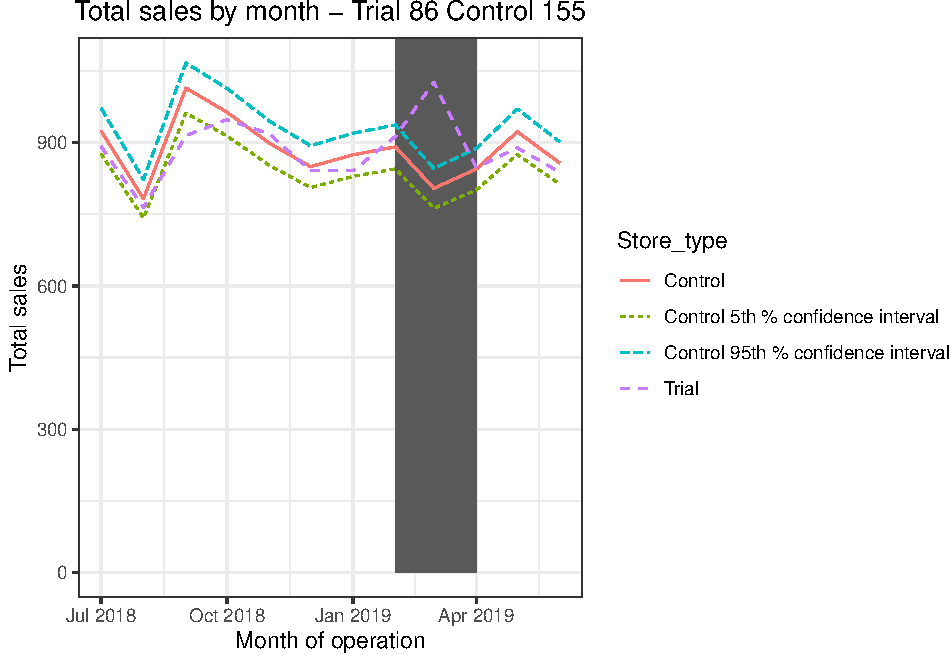
\includegraphics{Task2_files/figure-latex/unnamed-chunk-11-1}

The results show that the trial in store 86 is not significantly
different to its control store in the trial period as the trial store
performance lies inside the 5\% to 95\% confidence interval of the
control store in two of the three trial months.

Let's have a look at assessing this for the number of customers as well.

\begin{Shaded}
\begin{Highlighting}[]
\CommentTok{#### This would be a repeat of the steps before for total sales}
\CommentTok{#### Scale pre-trial control customers to match pre-trial trial store customers}
\NormalTok{scalingFactorForControlCust <-}\StringTok{ }\NormalTok{preTrialMeasures[STORE_NBR }\OperatorTok{==}\StringTok{ }\NormalTok{trial_store, }\KeywordTok{sum}\NormalTok{(nCustomers)]}\OperatorTok{/}
\StringTok{                               }\NormalTok{preTrialMeasures[STORE_NBR }\OperatorTok{==}\StringTok{ }\NormalTok{control_store, }\KeywordTok{sum}\NormalTok{(nCustomers)]}
\CommentTok{#### Apply the scaling factor}
\NormalTok{measureOverTimeCusts <-}\StringTok{ }\NormalTok{measureOverTime[, Store_type }\OperatorTok{:}\ErrorTok{=}\StringTok{ }\KeywordTok{ifelse}\NormalTok{(STORE_NBR }\OperatorTok{==}\StringTok{ }\NormalTok{trial_store, }\StringTok{'Trial'}\NormalTok{,}
                                                               \KeywordTok{ifelse}\NormalTok{(STORE_NBR }\OperatorTok{==}\StringTok{ }\NormalTok{control_store,}
                                                                      \StringTok{"Control"}\NormalTok{, }\StringTok{"Other stores"}\NormalTok{))]}
\CommentTok{# scaledControlCustomers <- measureOverTime %>%}
\CommentTok{#   filter(STORE_NBR == control_store) %>%}
\CommentTok{#   mutate(Store_type = ifelse(STORE_NBR == trial_store, "Trial",}
\CommentTok{#                              ifelse(STORE_NBR == control_store,}
\CommentTok{#                                     "Control", "Other stores")),}
\CommentTok{#          controlCustomers = nCustomers * scalingFactorForControlCust)}
\NormalTok{scaledControlCustomers <-}\StringTok{ }\NormalTok{measureOverTimeCusts[STORE_NBR }\OperatorTok{==}\StringTok{ }\NormalTok{control_store,}
\NormalTok{                                               ][ , controlCustomers }\OperatorTok{:}\ErrorTok{=}\StringTok{ }\NormalTok{nCustomers}
                                                  \OperatorTok{*}\StringTok{ }\NormalTok{scalingFactorForControlCust}
\NormalTok{                                                  ]}
\CommentTok{#### Calculate the percentage difference between scaled control customer and trial customer}
\NormalTok{percentageDiff <-}\StringTok{ }\KeywordTok{merge}\NormalTok{(scaledControlCustomers[, }\KeywordTok{c}\NormalTok{(}\StringTok{"YEARMONTH"}\NormalTok{, }\StringTok{"controlCustomers"}\NormalTok{)],}
\NormalTok{                        measureOverTime[STORE_NBR }\OperatorTok{==}\StringTok{ }\NormalTok{trial_store, }\KeywordTok{c}\NormalTok{(}\StringTok{"nCustomers"}\NormalTok{, }\StringTok{"YEARMONTH"}\NormalTok{)],}
                        \DataTypeTok{by =} \StringTok{"YEARMONTH"}
\NormalTok{                        )[, percentageDiff }\OperatorTok{:}\ErrorTok{=}\StringTok{ }\KeywordTok{abs}\NormalTok{(nCustomers}\OperatorTok{/}\NormalTok{controlCustomers}\DecValTok{-1}\NormalTok{)]}
\CommentTok{#### As our null hypothesis is that the trial period is the same as the pre-trial period, let's take the standard deviation based on the scaled percentage difference in the pre-trial period}
\NormalTok{stdDev <-}\StringTok{ }\KeywordTok{sd}\NormalTok{(percentageDiff[YEARMONTH }\OperatorTok{<}\StringTok{ }\DecValTok{201902}\NormalTok{ , percentageDiff])}
\NormalTok{degreesOfFreedom <-}\StringTok{ }\DecValTok{7}
\CommentTok{#### Trial and control store number of customers}
\NormalTok{pastCustomers <-}\StringTok{ }\NormalTok{measureOverTimeCusts[, nCusts }\OperatorTok{:}\ErrorTok{=}\StringTok{ }\KeywordTok{mean}\NormalTok{(nCustomers), by =}\StringTok{ }
\StringTok{                                        }\KeywordTok{c}\NormalTok{(}\StringTok{"YEARMONTH"}\NormalTok{, }\StringTok{"Store_type"}\NormalTok{)}
\NormalTok{                                      ][Store_type }\OperatorTok\StringTok{ }\KeywordTok{c}\NormalTok{(}\StringTok{"Trial"}\NormalTok{, }\StringTok{"Control"}\NormalTok{), ]}
\CommentTok{#### Control store 95th percentile}
\NormalTok{pastCustomers_Controls95 <-}\StringTok{ }\NormalTok{pastCustomers[Store_type }\OperatorTok{==}\StringTok{ "Control"}\NormalTok{,}
\NormalTok{                                          ][, nCusts }\OperatorTok{:}\ErrorTok{=}\StringTok{ }\NormalTok{nCusts }\OperatorTok{*}\StringTok{ }\NormalTok{(}\DecValTok{1} \OperatorTok{+}\StringTok{ }\NormalTok{stdDev }\OperatorTok{*}\StringTok{ }\DecValTok{2}\NormalTok{)}
\NormalTok{                                          ][, Store_type }\OperatorTok{:}\ErrorTok{=}\StringTok{ "Control 95th % confidence interval"}\NormalTok{]}
\CommentTok{#### Control store 5th percentile}
\NormalTok{pastCustomers_Controls5 <-}\StringTok{ }\NormalTok{pastCustomers[Store_type }\OperatorTok{==}\StringTok{ "Control"}\NormalTok{,}
\NormalTok{                                         ][, nCusts }\OperatorTok{:}\ErrorTok{=}\StringTok{ }\NormalTok{nCusts }\OperatorTok{*}\StringTok{ }\NormalTok{(}\DecValTok{1} \OperatorTok{-}\StringTok{ }\NormalTok{stdDev }\OperatorTok{*}\StringTok{ }\DecValTok{2}\NormalTok{)}
\NormalTok{                                         ][, Store_type }\OperatorTok{:}\ErrorTok{=}\StringTok{ "Control 5th % confidence interval"}\NormalTok{]}
\NormalTok{trialAssessment <-}\StringTok{ }\KeywordTok{rbind}\NormalTok{(pastCustomers, }
\NormalTok{                         pastCustomers_Controls95,}
\NormalTok{                         pastCustomers_Controls5}
\NormalTok{                         )[, TransactionMonth }\OperatorTok{:}\ErrorTok{=}\StringTok{ }\KeywordTok{as.Date}\NormalTok{(}\KeywordTok{paste}\NormalTok{(YEARMONTH }\OperatorTok\StringTok{ }\DecValTok{100}\NormalTok{,}
\NormalTok{                                                               YEARMONTH }\OperatorTok\StringTok{ }\DecValTok{100}\NormalTok{, }\DecValTok{1}\NormalTok{,}
                                                               \DataTypeTok{sep =} \StringTok{'-'}\NormalTok{))]}
\CommentTok{#### Plotting these in one nice graph}
\NormalTok{pp4<-}\KeywordTok{ggplot}\NormalTok{(trialAssessment, }\KeywordTok{aes}\NormalTok{(TransactionMonth, nCusts, }\DataTypeTok{color =}\NormalTok{ Store_type)) }\OperatorTok{+}
\StringTok{  }\KeywordTok{geom_rect}\NormalTok{(}\DataTypeTok{data =}\NormalTok{ trialAssessment[ YEARMONTH }\OperatorTok{<}\StringTok{ }\DecValTok{201905} \OperatorTok{&}\StringTok{ }\NormalTok{YEARMONTH }\OperatorTok{>}\StringTok{ }\DecValTok{201901}\NormalTok{ ,],}
            \KeywordTok{aes}\NormalTok{(}\DataTypeTok{xmin =} \KeywordTok{min}\NormalTok{(TransactionMonth), }\DataTypeTok{xmax =} \KeywordTok{max}\NormalTok{(TransactionMonth), }
                \DataTypeTok{ymin =} \DecValTok{0}\NormalTok{ , }\DataTypeTok{ymax =} \OtherTok{Inf}\NormalTok{, }\DataTypeTok{color =} \OtherTok{NULL}\NormalTok{), }\DataTypeTok{show.legend =} \OtherTok{FALSE}\NormalTok{) }\OperatorTok{+}
\StringTok{  }\KeywordTok{geom_line}\NormalTok{() }\OperatorTok{+}
\StringTok{  }\KeywordTok{labs}\NormalTok{(}\DataTypeTok{x =} \StringTok{"Month of operation"}\NormalTok{, }\DataTypeTok{y =} \StringTok{"Number of customers"}\NormalTok{, }
  \DataTypeTok{title =} \StringTok{"Total customers by month - Trial 86 Control 155"}\NormalTok{) }
\NormalTok{pp4}
\end{Highlighting}
\end{Shaded}

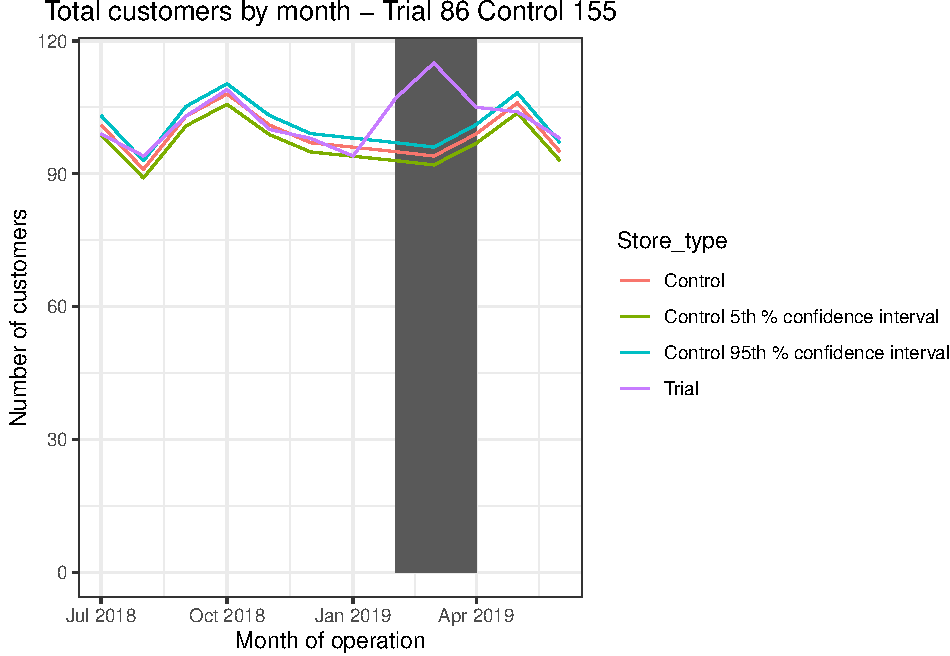
\includegraphics{Task2_files/figure-latex/unnamed-chunk-12-1}

It looks like the number of customers is significantly higher in all of
the three months. This seems to suggest that the trial had a significant
impact on increasing the number of customers in trial store 86 but as we
saw, sales were not significantly higher. We should check with the
Category Manager if there were special deals in the trial store that
were may have resulted in lower prices, impacting the results.

\hypertarget{trial-store-88}{%
\subsection{Trial store 88}\label{trial-store-88}}

\begin{Shaded}
\begin{Highlighting}[]
\CommentTok{#### All over to you now! Your manager has left for a conference call, so you'll be on your own this time.}
\CommentTok{#### Conduct the analysis on trial store 88.}
\NormalTok{measureOverTime <-}\StringTok{ }\NormalTok{data[, .(}\DataTypeTok{totSales =} \KeywordTok{sum}\NormalTok{(TOT_SALES),}
                            \DataTypeTok{nCustomers =} \KeywordTok{uniqueN}\NormalTok{(LYLTY_CARD_NBR),}
                            \DataTypeTok{nTxnPerCust =} \KeywordTok{uniqueN}\NormalTok{(TXN_ID)}\OperatorTok{/}\KeywordTok{uniqueN}\NormalTok{(LYLTY_CARD_NBR),}
                            \DataTypeTok{nChipsPerTxn =} \KeywordTok{sum}\NormalTok{(PROD_QTY)}\OperatorTok{/}\KeywordTok{uniqueN}\NormalTok{(TXN_ID),}
                            \DataTypeTok{avgPricePerUnit =} \KeywordTok{sum}\NormalTok{(TOT_SALES)}\OperatorTok{/}\KeywordTok{sum}\NormalTok{(PROD_QTY)}
\NormalTok{                            ), by =}\StringTok{ }\NormalTok{.(YEARMONTH, STORE_NBR)][}\KeywordTok{order}\NormalTok{(YEARMONTH, STORE_NBR)]}
\NormalTok{storesWithFullObs <-}\StringTok{ }\KeywordTok{unique}\NormalTok{(measureOverTime[, .N, }\DataTypeTok{by =}\NormalTok{ STORE_NBR][N}\OperatorTok{==}\DecValTok{12}\NormalTok{, STORE_NBR])}
\NormalTok{preTrialMeasures <-}\StringTok{ }\NormalTok{measureOverTime[YEARMONTH}\OperatorTok{<}\DecValTok{201902} \OperatorTok{&}\StringTok{ }\NormalTok{STORE_NBR }\OperatorTok\StringTok{ }\NormalTok{storesWithFullObs,]}

\CommentTok{#### Use the functions from earlier to calculate the correlation of the sales and number of customers of each potential control store to the trial store}
\NormalTok{trial_store <-}\StringTok{ }\DecValTok{88}
\NormalTok{corr_nSales <-}\StringTok{ }\KeywordTok{calculateCorrelation}\NormalTok{(preTrialMeasures, }\KeywordTok{quote}\NormalTok{(totSales), trial_store)}
\NormalTok{corr_nCustomers <-}\StringTok{ }\KeywordTok{calculateCorrelation}\NormalTok{(preTrialMeasures, }\KeywordTok{quote}\NormalTok{(nCustomers), trial_store)}
\CommentTok{#### Use the functions from earlier to calculate the magnitude distance of the sales and number of customers of each potential control store to the trial store}
\NormalTok{magnitude_nSales <-}\StringTok{ }\KeywordTok{calculateMagnitudeDistance}\NormalTok{(preTrialMeasures, }\KeywordTok{quote}\NormalTok{(totSales), trial_store)}
\NormalTok{magnitude_nCustomers <-}\StringTok{ }\KeywordTok{calculateMagnitudeDistance}\NormalTok{(preTrialMeasures, }\KeywordTok{quote}\NormalTok{(nCustomers), trial_store)}
\CommentTok{#### Create a combined score composed of correlation and magnitude by merging the correlations table and the magnitudes table, for each driver.}
\NormalTok{corr_weight <-}\StringTok{ }\FloatTok{0.5}
\NormalTok{score_nSales <-}\StringTok{ }\KeywordTok{merge}\NormalTok{(corr_nSales, magnitude_nSales,}
                      \DataTypeTok{by =} \KeywordTok{c}\NormalTok{(}\StringTok{'Store1'}\NormalTok{, }\StringTok{'Store2'}\NormalTok{)}
\NormalTok{                      )[, scoreNSales }\OperatorTok{:}\ErrorTok{=}\StringTok{ }\NormalTok{corr_weight}\OperatorTok{*}\NormalTok{corr_measure}\OperatorTok{+}\NormalTok{(}\DecValTok{1}\OperatorTok{-}\NormalTok{corr_weight)}\OperatorTok{*}\NormalTok{mag_measure]}
\NormalTok{score_nCustomers <-}\StringTok{ }\KeywordTok{merge}\NormalTok{(corr_nCustomers, magnitude_nCustomers,}
                      \DataTypeTok{by =} \KeywordTok{c}\NormalTok{(}\StringTok{'Store1'}\NormalTok{, }\StringTok{'Store2'}\NormalTok{)}
\NormalTok{                      )[, scoreNCust }\OperatorTok{:}\ErrorTok{=}\StringTok{ }\NormalTok{corr_weight}\OperatorTok{*}\NormalTok{corr_measure}\OperatorTok{+}\NormalTok{(}\DecValTok{1}\OperatorTok{-}\NormalTok{corr_weight)}\OperatorTok{*}\NormalTok{mag_measure]}
\CommentTok{#### Combine scores across the drivers by merging sales scores and customer scores, and compute a final combined score.}
\NormalTok{score_Control <-}\StringTok{ }\KeywordTok{merge}\NormalTok{(score_nSales, score_nCustomers, }\DataTypeTok{by =} \KeywordTok{c}\NormalTok{(}\StringTok{'Store1'}\NormalTok{, }\StringTok{'Store2'}\NormalTok{))}
\NormalTok{score_Control[, finalControlScore }\OperatorTok{:}\ErrorTok{=}\StringTok{ }\NormalTok{(scoreNSales}\OperatorTok{+}\NormalTok{scoreNCust)}\OperatorTok{/}\DecValTok{2}\NormalTok{]}
\CommentTok{#### Select control stores based on the highest matching store}
\CommentTok{#### (closest to 1 but not the store itself, i.e. the second ranked highest store)}
\CommentTok{#### Select control store for trial store 88}
\NormalTok{control_store <-}\StringTok{ }\NormalTok{score_Control[}\KeywordTok{order}\NormalTok{(}\OperatorTok{-}\NormalTok{finalControlScore)][}\DecValTok{2}\NormalTok{, Store2]}
\NormalTok{control_store}
\end{Highlighting}
\end{Shaded}

\begin{verbatim}
## [1] 237
\end{verbatim}

We've now found store 237 to be a suitable control store for trial store
88.

Again, let's check visually if the drivers are indeed similar in the
period before the trial.

We'll look at total sales first.

\begin{Shaded}
\begin{Highlighting}[]
\CommentTok{#### Visual checks on trends based on the drivers}
\CommentTok{#### For the period before the trial, create a graph with total sales of the trial store for each month, compared to the control store and other stores.}
\NormalTok{measureOverTimeSales <-}\StringTok{ }\NormalTok{measureOverTime}
\NormalTok{pastSales <-}\StringTok{ }\NormalTok{measureOverTime }\OperatorTok
\StringTok{  }\KeywordTok{mutate}\NormalTok{(}\DataTypeTok{Store_type =} \KeywordTok{ifelse}\NormalTok{(STORE_NBR}\OperatorTok{==}\NormalTok{control_store, }\StringTok{'Control'}\NormalTok{,}
                             \KeywordTok{ifelse}\NormalTok{(STORE_NBR}\OperatorTok{==}\NormalTok{trial_store, }\StringTok{'Trial'}\NormalTok{,}
                                    \StringTok{'Other store'}\NormalTok{))) }\OperatorTok
\StringTok{  }\KeywordTok{group_by}\NormalTok{(YEARMONTH, Store_type) }\OperatorTok
\StringTok{  }\KeywordTok{summarise}\NormalTok{(}\DataTypeTok{totSales =} \KeywordTok{mean}\NormalTok{(totSales), }\DataTypeTok{.groups=}\StringTok{'drop'}\NormalTok{) }\OperatorTok
\StringTok{  }\KeywordTok{mutate}\NormalTok{(}\DataTypeTok{TransactionMonth =} \KeywordTok{as.Date}\NormalTok{(}\KeywordTok{paste}\NormalTok{(YEARMONTH }\OperatorTok\StringTok{ }\DecValTok{100}\NormalTok{,}
\NormalTok{                                          YEARMONTH }\OperatorTok\StringTok{ }\DecValTok{100}\NormalTok{, }\DecValTok{1}\NormalTok{,}
                                          \DataTypeTok{sep =} \StringTok{'-'}\NormalTok{))) }\OperatorTok
\StringTok{  }\KeywordTok{filter}\NormalTok{(YEARMONTH }\OperatorTok{<}\DecValTok{201902}\NormalTok{)}
\NormalTok{p5<-}\KeywordTok{ggplot}\NormalTok{(pastSales, }\KeywordTok{aes}\NormalTok{(TransactionMonth, totSales, }\DataTypeTok{color =}\NormalTok{ Store_type)) }\OperatorTok{+}
\KeywordTok{geom_line}\NormalTok{() }\OperatorTok{+}
\KeywordTok{labs}\NormalTok{(}\DataTypeTok{x=}\StringTok{'Month of operation'}\NormalTok{, }\DataTypeTok{y =} \StringTok{'Total sales'}\NormalTok{, }
     \DataTypeTok{title=}\StringTok{'    Trial 88 vs Control 237}
\StringTok{     Total sales by month'}\NormalTok{)}
\NormalTok{p5}
\end{Highlighting}
\end{Shaded}

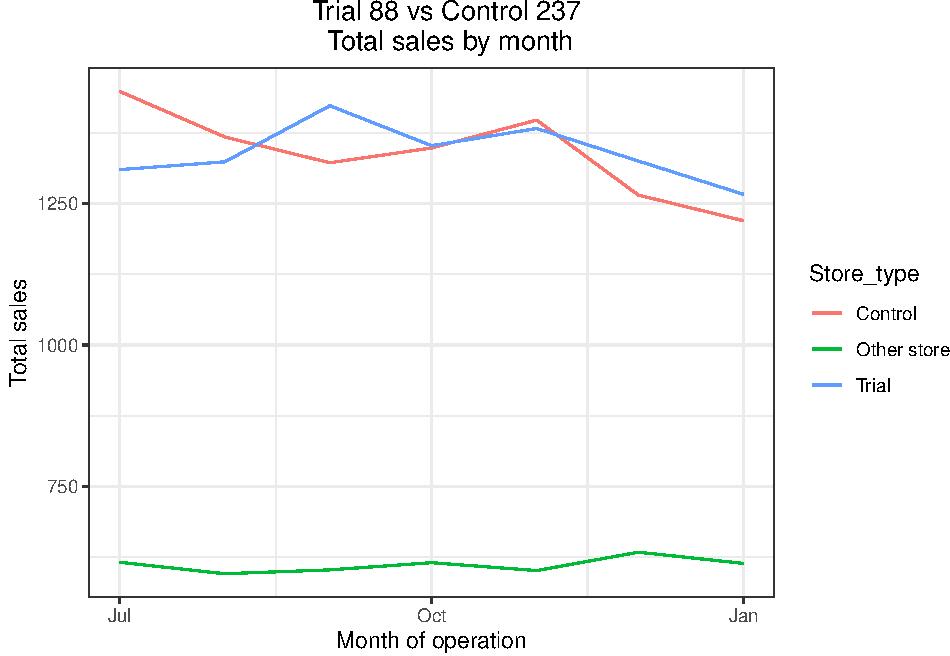
\includegraphics{Task2_files/figure-latex/unnamed-chunk-14-1.pdf} Great,
the trial and control stores have similar total sales.

Next, number of customers.

\begin{Shaded}
\begin{Highlighting}[]
\CommentTok{#### Visual checks on trends based on the drivers}
\CommentTok{#### For the period before the trial, create a graph with customer counts of the trial store for each month, compared to the control store and other stores.}
\NormalTok{measureOverTimeCusts <-}\StringTok{ }\NormalTok{measureOverTime}
\NormalTok{pastCustomers <-}\StringTok{ }\NormalTok{measureOverTime }\OperatorTok
\StringTok{  }\KeywordTok{mutate}\NormalTok{(}\DataTypeTok{Store_type =} \KeywordTok{ifelse}\NormalTok{(STORE_NBR}\OperatorTok{==}\NormalTok{control_store, }\StringTok{'Control'}\NormalTok{,}
                             \KeywordTok{ifelse}\NormalTok{(STORE_NBR}\OperatorTok{==}\NormalTok{trial_store, }\StringTok{'Trial'}\NormalTok{,}
                                    \StringTok{'Other stores'}\NormalTok{))) }\OperatorTok
\StringTok{  }\KeywordTok{group_by}\NormalTok{(YEARMONTH, Store_type) }\OperatorTok
\StringTok{  }\KeywordTok{summarise}\NormalTok{(}\DataTypeTok{nCustomers =} \KeywordTok{mean}\NormalTok{(nCustomers), }\DataTypeTok{.groups=}\StringTok{'drop'}\NormalTok{) }\OperatorTok
\StringTok{  }\KeywordTok{mutate}\NormalTok{(}\DataTypeTok{TransactionMonth =} \KeywordTok{as.Date}\NormalTok{(}\KeywordTok{paste}\NormalTok{(YEARMONTH }\OperatorTok\StringTok{ }\DecValTok{100}\NormalTok{,}
\NormalTok{                                          YEARMONTH }\OperatorTok\StringTok{ }\DecValTok{100}\NormalTok{, }\DecValTok{1}\NormalTok{,}
                                          \DataTypeTok{sep =} \StringTok{'-'}\NormalTok{))) }\OperatorTok
\StringTok{  }\KeywordTok{filter}\NormalTok{(YEARMONTH }\OperatorTok{<}\DecValTok{201902}\NormalTok{)}
\NormalTok{p6<-}\KeywordTok{ggplot}\NormalTok{(pastCustomers, }\KeywordTok{aes}\NormalTok{(TransactionMonth, nCustomers, }\DataTypeTok{color=}\NormalTok{Store_type)) }\OperatorTok{+}
\KeywordTok{geom_line}\NormalTok{() }\OperatorTok{+}
\KeywordTok{labs}\NormalTok{(}\DataTypeTok{x=}\StringTok{'Month of operation'}\NormalTok{, }\DataTypeTok{y=}\StringTok{'Number of customers'}\NormalTok{, }
     \DataTypeTok{title =} \StringTok{'    Trial 88 vs Control 237}
\StringTok{     Total customers by month'}\NormalTok{)}
\NormalTok{p6}
\end{Highlighting}
\end{Shaded}

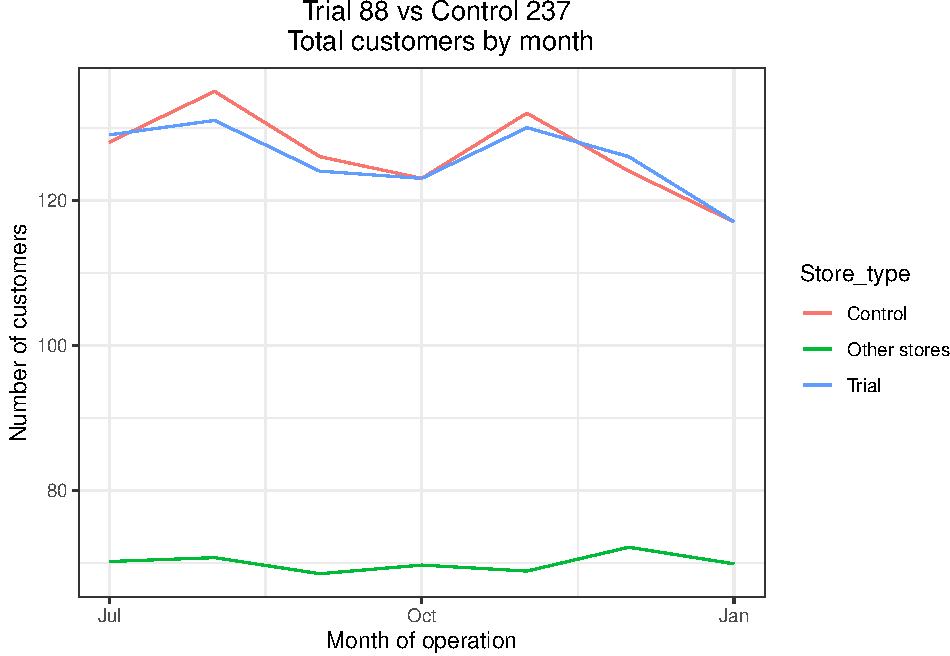
\includegraphics{Task2_files/figure-latex/unnamed-chunk-15-1.pdf} Total
number of customers of the control and trial stores are also similar.

Let's now assess the impact of the trial on sales.

\begin{Shaded}
\begin{Highlighting}[]
\CommentTok{#### Scale pre-trial control store sales to match pre-trial trial store sales}
\NormalTok{scalingFactorForControlSales <-}\StringTok{ }\NormalTok{preTrialMeasures[STORE_NBR}\OperatorTok{==}\NormalTok{trial_store, }\KeywordTok{sum}\NormalTok{(totSales)]}\OperatorTok{/}
\StringTok{                                }\NormalTok{preTrialMeasures[STORE_NBR}\OperatorTok{==}\NormalTok{control_store, }\KeywordTok{sum}\NormalTok{(totSales)]}
\CommentTok{#### Apply the scaling factor}
\NormalTok{measureOverTimeSales <-}\StringTok{ }\NormalTok{measureOverTime}
\NormalTok{scaledControlSales <-}\StringTok{ }\NormalTok{measureOverTime[STORE_NBR}\OperatorTok{==}\NormalTok{control_store, }
\NormalTok{                                      ][, controlSales }\OperatorTok{:}\ErrorTok{=}\StringTok{ }\NormalTok{totSales}\OperatorTok{*}\NormalTok{scalingFactorForControlSales]}
\CommentTok{#### Calculate the absolute percentage difference between scaled control sales and trial sales}
\NormalTok{percentageDiff <-}\StringTok{ }\KeywordTok{merge}\NormalTok{(scaledControlSales[,}\KeywordTok{c}\NormalTok{(}\StringTok{'YEARMONTH'}\NormalTok{,}\StringTok{'controlSales'}\NormalTok{)], }
\NormalTok{                        measureOverTimeSales[STORE_NBR}\OperatorTok{==}\StringTok{ }\NormalTok{trial_store, }\KeywordTok{c}\NormalTok{(}\StringTok{'YEARMONTH'}\NormalTok{, }\StringTok{'totSales'}\NormalTok{)], }
                        \DataTypeTok{by=} \StringTok{'YEARMONTH'}\NormalTok{)[, percentageDiff }\OperatorTok{:}\ErrorTok{=}\StringTok{ }\KeywordTok{abs}\NormalTok{(totSales}\OperatorTok{/}\NormalTok{controlSales}\DecValTok{-1}\NormalTok{)]}
\CommentTok{#### As our null hypothesis is that the trial period is the same as the pre-trial period, let's take the standard deviation based on the scaled percentage difference in the pre-trial period}
\NormalTok{stdDev <-}\StringTok{ }\KeywordTok{sd}\NormalTok{(percentageDiff[YEARMONTH}\OperatorTok{<}\DecValTok{201902}\NormalTok{, percentageDiff])}

\NormalTok{degreesOfFreedom <-}\StringTok{ }\DecValTok{7}
\CommentTok{#### Trial and control store total sales}
\NormalTok{measureOverTimeSales <-}\StringTok{ }\NormalTok{measureOverTime}
\NormalTok{pastSales <-}\StringTok{ }\NormalTok{measureOverTime }\OperatorTok
\StringTok{  }\KeywordTok{mutate}\NormalTok{(}\DataTypeTok{Store_type =} \KeywordTok{ifelse}\NormalTok{(STORE_NBR}\OperatorTok{==}\NormalTok{control_store, }\StringTok{'Control'}\NormalTok{,}
                             \KeywordTok{ifelse}\NormalTok{(STORE_NBR}\OperatorTok{==}\NormalTok{trial_store, }\StringTok{'Trial'}\NormalTok{,}
                                    \StringTok{'Other stores'}\NormalTok{))) }\OperatorTok
\StringTok{  }\KeywordTok{filter}\NormalTok{(Store_type }\OperatorTok\StringTok{ }\KeywordTok{c}\NormalTok{(}\StringTok{'Trial'}\NormalTok{, }\StringTok{'Control'}\NormalTok{)) }\OperatorTok
\StringTok{  }\KeywordTok{group_by}\NormalTok{(YEARMONTH, Store_type) }\OperatorTok
\StringTok{  }\KeywordTok{summarise}\NormalTok{(}\DataTypeTok{totSales =} \KeywordTok{mean}\NormalTok{(totSales), }\DataTypeTok{.groups=}\StringTok{'drop'}\NormalTok{) }\OperatorTok
\StringTok{  }\KeywordTok{mutate}\NormalTok{(}\DataTypeTok{TransactionMonth =} \KeywordTok{as.Date}\NormalTok{(}\KeywordTok{paste}\NormalTok{(YEARMONTH }\OperatorTok\StringTok{ }\DecValTok{100}\NormalTok{,}
\NormalTok{                                          YEARMONTH }\OperatorTok\StringTok{ }\DecValTok{100}\NormalTok{, }\DecValTok{1}\NormalTok{,}
                                          \DataTypeTok{sep =} \StringTok{'-'}\NormalTok{)))}
\CommentTok{#### Control store 95th percentile}
\NormalTok{pastSales_Controls95 <-}\StringTok{ }\NormalTok{pastSales }\OperatorTok
\StringTok{  }\KeywordTok{filter}\NormalTok{(Store_type}\OperatorTok{==}\StringTok{'Control'}\NormalTok{) }\OperatorTok
\StringTok{  }\KeywordTok{mutate}\NormalTok{(}\DataTypeTok{totSales =}\NormalTok{ totSales}\OperatorTok{*}\NormalTok{(}\DecValTok{1} \OperatorTok{+}\StringTok{ }\NormalTok{stdDev}\OperatorTok{*}\DecValTok{2}\NormalTok{),}
         \DataTypeTok{Store_type=} \StringTok{'Control 95th % confidence interval'}\NormalTok{)}
\CommentTok{#### Control store 5th percentile}
\NormalTok{pastSales_Controls5 <-}\StringTok{ }\NormalTok{pastSales }\OperatorTok
\StringTok{  }\KeywordTok{filter}\NormalTok{(Store_type}\OperatorTok{==}\StringTok{'Control'}\NormalTok{) }\OperatorTok
\StringTok{  }\KeywordTok{mutate}\NormalTok{(}\DataTypeTok{totSales =}\NormalTok{ totSales}\OperatorTok{*}\NormalTok{(}\DecValTok{1} \OperatorTok{-}\StringTok{ }\NormalTok{stdDev}\OperatorTok{*}\DecValTok{2}\NormalTok{),}
         \DataTypeTok{Store_type=} \StringTok{'Control 5th % confidence interval'}\NormalTok{)}
\CommentTok{#### Combine the tables pastSales, pastSales_Controls95, pastSales_Controls5}
\NormalTok{trialAssessment <-}\StringTok{ }\KeywordTok{rbind}\NormalTok{(pastSales, pastSales_Controls95, pastSales_Controls5)}
\CommentTok{#### Plot these in one nice graph}
\NormalTok{pp5<-}\KeywordTok{ggplot}\NormalTok{(trialAssessment, }\KeywordTok{aes}\NormalTok{(TransactionMonth, totSales, }\DataTypeTok{color=}\NormalTok{Store_type)) }\OperatorTok{+}
\KeywordTok{geom_rect}\NormalTok{(}\DataTypeTok{data =}\NormalTok{ trialAssessment }\OperatorTok\StringTok{ }\KeywordTok{filter}\NormalTok{(YEARMONTH}\OperatorTok{<}\DecValTok{201905} \OperatorTok{&}\StringTok{ }\NormalTok{YEARMONTH}\OperatorTok{>}\DecValTok{201901}\NormalTok{), }
          \KeywordTok{aes}\NormalTok{(}\DataTypeTok{xmin =} \KeywordTok{min}\NormalTok{(TransactionMonth), }\DataTypeTok{xmax =} \KeywordTok{max}\NormalTok{(TransactionMonth),}
          \DataTypeTok{ymin =} \DecValTok{0}\NormalTok{, }\DataTypeTok{ymax =} \OtherTok{Inf}\NormalTok{, }\DataTypeTok{color =} \OtherTok{NULL}\NormalTok{), }\DataTypeTok{show.legend =}\OtherTok{FALSE}\NormalTok{ )}\OperatorTok{+}
\KeywordTok{geom_line}\NormalTok{() }\OperatorTok{+}
\KeywordTok{labs}\NormalTok{(}\DataTypeTok{x =} \StringTok{'Month of operation'}\NormalTok{, }\DataTypeTok{y=}\StringTok{'Total sales'}\NormalTok{, }
     \DataTypeTok{title=}\StringTok{'Total sales by month - Trial 88 Control 237'}\NormalTok{)}
\NormalTok{pp5}
\end{Highlighting}
\end{Shaded}

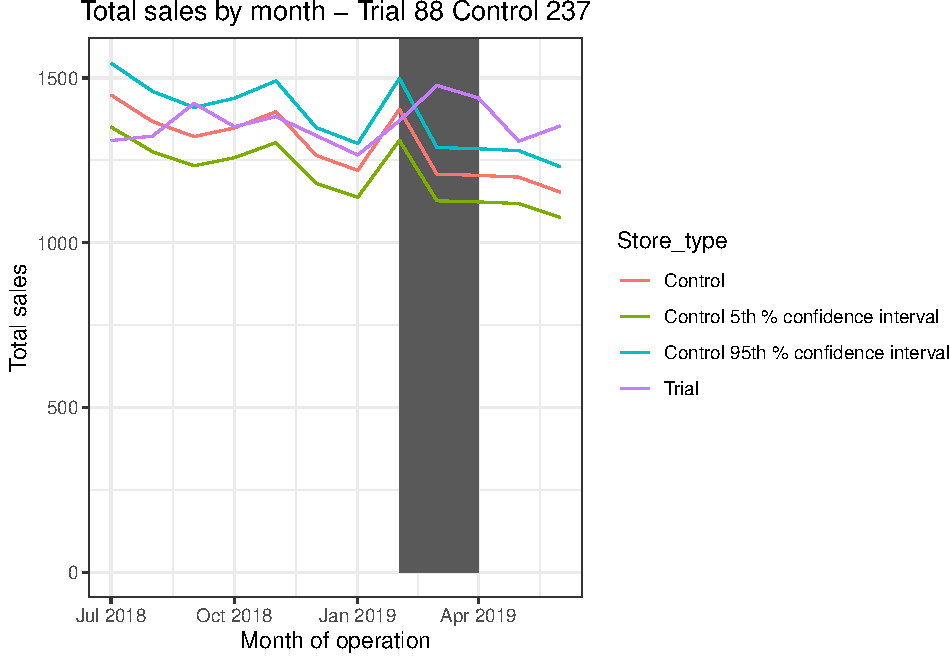
\includegraphics{Task2_files/figure-latex/unnamed-chunk-16-1}

The results show that the trial in store 88 is significantly different
to its control store in the trial period as the trial store performance
lies outside of the 5\% to 95\% confidence interval of the control store
in two of the three trial months.

Let's have a look at assessing this for number of customers as well.

\begin{Shaded}
\begin{Highlighting}[]
\CommentTok{#### This would be a repeat of the steps before for total sales}
\CommentTok{#### Scale pre-trial control store customers to match pre-trial trial store customers}
\NormalTok{scalingFactorForControlCust <-}\StringTok{ }\NormalTok{preTrialMeasures[STORE_NBR}\OperatorTok{==}\NormalTok{trial_store, }\KeywordTok{sum}\NormalTok{(nCustomers)]}\OperatorTok{/}
\StringTok{                               }\NormalTok{preTrialMeasures[STORE_NBR}\OperatorTok{==}\NormalTok{control_store, }\KeywordTok{sum}\NormalTok{(nCustomers)]}
\CommentTok{#### Apply the scaling factor}
\NormalTok{measureOverTimeCusts <-}\StringTok{ }\NormalTok{measureOverTime}
\NormalTok{scaledControlCustomers <-}\StringTok{ }\NormalTok{measureOverTimeCusts[STORE_NBR}\OperatorTok{==}\NormalTok{control_store,}
\NormalTok{                                               ][, controlCust }\OperatorTok{:}\ErrorTok{=}\StringTok{ }\NormalTok{nCustomers}\OperatorTok{*}
\StringTok{                                                   }\NormalTok{scalingFactorForControlCust]}
\CommentTok{#### Calculate the absolute percentage difference between scaled control sales and trial sales}
\NormalTok{percentageDiff <-}\StringTok{ }\KeywordTok{merge}\NormalTok{(scaledControlCustomers[,}\KeywordTok{c}\NormalTok{(}\StringTok{'YEARMONTH'}\NormalTok{, }\StringTok{'controlCust'}\NormalTok{)], }
\NormalTok{                        measureOverTimeCusts[STORE_NBR}\OperatorTok{==}\NormalTok{trial_store,}
                                             \KeywordTok{c}\NormalTok{(}\StringTok{'YEARMONTH'}\NormalTok{, }\StringTok{'nCustomers'}\NormalTok{)],}
                        \DataTypeTok{by =} \StringTok{'YEARMONTH'}\NormalTok{)[, percentageDiff}\OperatorTok{:}\ErrorTok{=}\StringTok{ }\KeywordTok{abs}\NormalTok{(nCustomers}\OperatorTok{/}\NormalTok{controlCust}\DecValTok{-1}\NormalTok{)]}
\CommentTok{#### As our null hypothesis is that the trial period is the same as the pre-trial period, let's take the standard deviation based on the scaled percentage difference in the pre-trial period}
\NormalTok{stdDev <-}\StringTok{ }\KeywordTok{sd}\NormalTok{(percentageDiff[YEARMONTH}\OperatorTok{<}\DecValTok{201902}\NormalTok{, percentageDiff])}
\NormalTok{degreesOfFreedom <-}\StringTok{ }\DecValTok{7} \CommentTok{# note that there are 8 months in the pre-trial period hence 8 - 1 = 7 degrees of freedom}
\CommentTok{#### Trial and control store number of customers}
\NormalTok{pastCustomers <-}\StringTok{ }\NormalTok{measureOverTimeCusts }\OperatorTok
\StringTok{  }\KeywordTok{mutate}\NormalTok{(}\DataTypeTok{Store_type =} \KeywordTok{ifelse}\NormalTok{(STORE_NBR}\OperatorTok{==}\NormalTok{control_store, }\StringTok{'Control'}\NormalTok{,}
                             \KeywordTok{ifelse}\NormalTok{(STORE_NBR}\OperatorTok{==}\NormalTok{trial_store, }\StringTok{'Trial'}\NormalTok{,}
                                    \StringTok{'Other stores'}\NormalTok{))) }\OperatorTok
\StringTok{  }\KeywordTok{filter}\NormalTok{(Store_type }\OperatorTok\StringTok{ }\KeywordTok{c}\NormalTok{(}\StringTok{'Trial'}\NormalTok{, }\StringTok{'Control'}\NormalTok{)) }\OperatorTok
\StringTok{  }\KeywordTok{group_by}\NormalTok{(YEARMONTH, Store_type) }\OperatorTok
\StringTok{  }\KeywordTok{summarise}\NormalTok{(}\DataTypeTok{nCustomers =} \KeywordTok{mean}\NormalTok{(nCustomers), }\DataTypeTok{.groups=}\StringTok{'drop'}\NormalTok{) }\OperatorTok
\StringTok{  }\KeywordTok{mutate}\NormalTok{(}\DataTypeTok{TransactionMonth =} \KeywordTok{as.Date}\NormalTok{(}\KeywordTok{paste}\NormalTok{(YEARMONTH }\OperatorTok\StringTok{ }\DecValTok{100}\NormalTok{,}
\NormalTok{                                          YEARMONTH }\OperatorTok\StringTok{ }\DecValTok{100}\NormalTok{, }\DecValTok{1}\NormalTok{,}
                                          \DataTypeTok{sep =} \StringTok{'-'}\NormalTok{)))}
\CommentTok{#### Control store 95th percentile}
\NormalTok{pastCustomers_Controls95 <-}\StringTok{ }\NormalTok{pastCustomers }\OperatorTok
\StringTok{  }\KeywordTok{filter}\NormalTok{(Store_type}\OperatorTok{==}\StringTok{'Control'}\NormalTok{) }\OperatorTok
\StringTok{  }\KeywordTok{mutate}\NormalTok{(}\DataTypeTok{nCustomers =}\NormalTok{ nCustomers }\OperatorTok{*}\StringTok{ }\NormalTok{(}\DecValTok{1}\OperatorTok{+}\NormalTok{stdDev}\OperatorTok{*}\DecValTok{2}\NormalTok{),}
         \DataTypeTok{Store_type =} \StringTok{'Control 95th % confidence interval'}\NormalTok{)}
\CommentTok{#### Control store 5th percentile}
\NormalTok{pastCustomers_Controls5 <-}\StringTok{ }\NormalTok{pastCustomers }\OperatorTok
\StringTok{  }\KeywordTok{filter}\NormalTok{(Store_type}\OperatorTok{==}\StringTok{'Control'}\NormalTok{) }\OperatorTok
\StringTok{  }\KeywordTok{mutate}\NormalTok{(}\DataTypeTok{nCustomers =}\NormalTok{ nCustomers }\OperatorTok{*}\StringTok{ }\NormalTok{(}\DecValTok{1}\OperatorTok{-}\NormalTok{stdDev}\OperatorTok{*}\DecValTok{2}\NormalTok{),}
         \DataTypeTok{Store_type =} \StringTok{'Control 5th % confidence interval'}\NormalTok{)}
\CommentTok{#### Combine the tables pastSales, pastSales_Controls95, pastSales_Controls5}
\NormalTok{trialAssessment <-}\StringTok{ }\KeywordTok{rbind}\NormalTok{(pastCustomers, pastCustomers_Controls95, pastCustomers_Controls5)}
\CommentTok{#### Plotting these in one nice graph}
\NormalTok{pp6<-}\KeywordTok{ggplot}\NormalTok{(trialAssessment, }\KeywordTok{aes}\NormalTok{(TransactionMonth, nCustomers, }\DataTypeTok{color =}\NormalTok{ Store_type)) }\OperatorTok{+}
\KeywordTok{geom_rect}\NormalTok{(}\DataTypeTok{data =}\NormalTok{ trialAssessment }\OperatorTok\StringTok{ }\KeywordTok{filter}\NormalTok{(YEARMONTH}\OperatorTok{<}\DecValTok{201905} \OperatorTok{&}\StringTok{ }\NormalTok{YEARMONTH}\OperatorTok{>}\DecValTok{201901}\NormalTok{),}
          \KeywordTok{aes}\NormalTok{(}\DataTypeTok{xmin=}\KeywordTok{min}\NormalTok{(TransactionMonth), }\DataTypeTok{xmax=}\KeywordTok{max}\NormalTok{(TransactionMonth),}
              \DataTypeTok{ymin=}\DecValTok{0}\NormalTok{, }\DataTypeTok{ymax=}\OtherTok{Inf}\NormalTok{, }\DataTypeTok{color=}\OtherTok{NULL}\NormalTok{), }\DataTypeTok{show.legend =} \OtherTok{FALSE}\NormalTok{) }\OperatorTok{+}
\KeywordTok{geom_line}\NormalTok{() }\OperatorTok{+}
\KeywordTok{labs}\NormalTok{(}\DataTypeTok{x=}\StringTok{'Month of operation'}\NormalTok{, }\DataTypeTok{y=}\StringTok{'Number of customers'}\NormalTok{, }
     \DataTypeTok{title =} \StringTok{'Total customers by month - Trial 88 Control 237'}\NormalTok{)}
\NormalTok{pp6}
\end{Highlighting}
\end{Shaded}

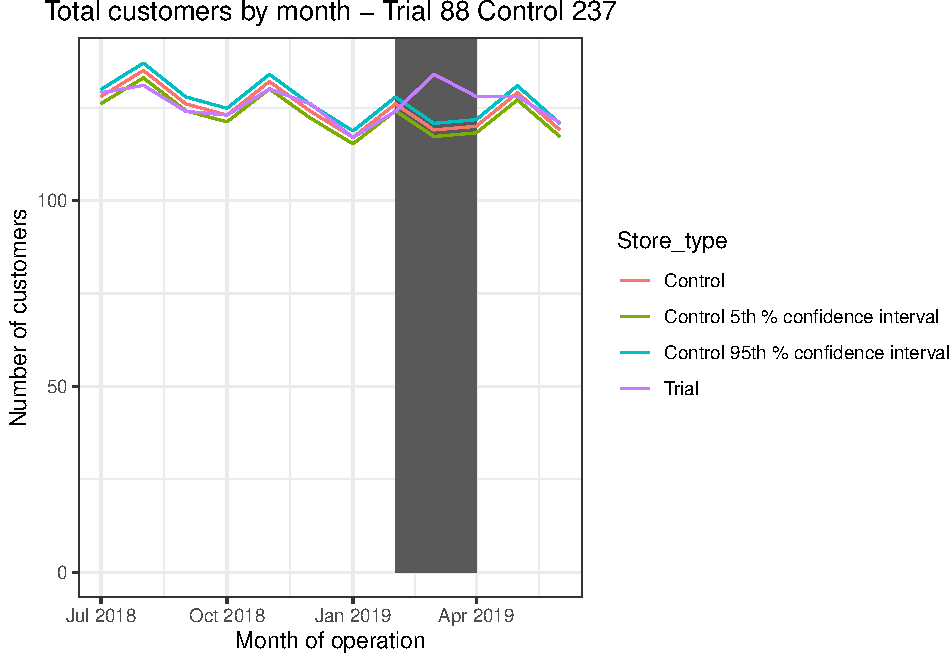
\includegraphics{Task2_files/figure-latex/unnamed-chunk-17-1}

Total number of customers in the trial period for the trial store is
significantly higher than the control store for two out of three months,
which indicates a positive trial effect.

\hypertarget{conclusion}{%
\subsection{Conclusion}\label{conclusion}}

Good work! We've found control stores 233, 155, 237 for trial stores 77,
86 and 88 respectively.

The results for trial stores 77 and 88 during the trial period show a
significant difference in at least two of the three trial months but
this is not the case for trial store 86. We can check with the client if
the implementation of the trial was different in trial store 86 but
overall, the trial shows a significant increase in sales. Now that we
have finished our analysis, we can prepare our presentation to the
Category Manager.

\begin{Shaded}
\begin{Highlighting}[]
\CommentTok{# Define multiple plot function}
\CommentTok{#}
\CommentTok{# ggplot objects can be passed in ..., or to plotlist (as a list of ggplot objects)}
\CommentTok{# - cols:   Number of columns in layout}
\CommentTok{# - layout: A matrix specifying the layout. If present, 'cols' is ignored.}
\CommentTok{#}
\CommentTok{# If the layout is something like matrix(c(1,2,3,3), nrow=2, byrow=TRUE),}
\CommentTok{# then plot 1 will go in the upper left, 2 will go in the upper right, and}
\CommentTok{# 3 will go all the way across the bottom.}
\CommentTok{#}
\NormalTok{multiplot <-}\StringTok{ }\ControlFlowTok{function}\NormalTok{(..., }\DataTypeTok{plotlist=}\OtherTok{NULL}\NormalTok{, file, }\DataTypeTok{cols=}\DecValTok{1}\NormalTok{, }\DataTypeTok{layout=}\OtherTok{NULL}\NormalTok{) \{}

  \CommentTok{# Make a list from the ... arguments and plotlist}
\NormalTok{  plots <-}\StringTok{ }\KeywordTok{c}\NormalTok{(}\KeywordTok{list}\NormalTok{(...), plotlist)}

\NormalTok{  numPlots =}\StringTok{ }\KeywordTok{length}\NormalTok{(plots)}

  \CommentTok{# If layout is NULL, then use 'cols' to determine layout}
  \ControlFlowTok{if}\NormalTok{ (}\KeywordTok{is.null}\NormalTok{(layout)) \{}
    \CommentTok{# Make the panel}
    \CommentTok{# ncol: Number of columns of plots}
    \CommentTok{# nrow: Number of rows needed, calculated from # of cols}
\NormalTok{    layout <-}\StringTok{ }\KeywordTok{matrix}\NormalTok{(}\KeywordTok{seq}\NormalTok{(}\DecValTok{1}\NormalTok{, cols }\OperatorTok{*}\StringTok{ }\KeywordTok{ceiling}\NormalTok{(numPlots}\OperatorTok{/}\NormalTok{cols)),}
                    \DataTypeTok{ncol =}\NormalTok{ cols, }\DataTypeTok{nrow =} \KeywordTok{ceiling}\NormalTok{(numPlots}\OperatorTok{/}\NormalTok{cols))}
\NormalTok{  \}}

 \ControlFlowTok{if}\NormalTok{ (numPlots}\OperatorTok{==}\DecValTok{1}\NormalTok{) \{}
    \KeywordTok{print}\NormalTok{(plots[[}\DecValTok{1}\NormalTok{]])}

\NormalTok{  \} }\ControlFlowTok{else}\NormalTok{ \{}
    \CommentTok{# Set up the page}
    \KeywordTok{grid.newpage}\NormalTok{()}
    \KeywordTok{pushViewport}\NormalTok{(}\KeywordTok{viewport}\NormalTok{(}\DataTypeTok{layout =} \KeywordTok{grid.layout}\NormalTok{(}\KeywordTok{nrow}\NormalTok{(layout), }\KeywordTok{ncol}\NormalTok{(layout))))}

    \CommentTok{# Make each plot, in the correct location}
    \ControlFlowTok{for}\NormalTok{ (i }\ControlFlowTok{in} \DecValTok{1}\OperatorTok{:}\NormalTok{numPlots) \{}
      \CommentTok{# Get the i,j matrix positions of the regions that contain this subplot}
\NormalTok{      matchidx <-}\StringTok{ }\KeywordTok{as.data.frame}\NormalTok{(}\KeywordTok{which}\NormalTok{(layout }\OperatorTok{==}\StringTok{ }\NormalTok{i, }\DataTypeTok{arr.ind =} \OtherTok{TRUE}\NormalTok{))}

      \KeywordTok{print}\NormalTok{(plots[[i]], }\DataTypeTok{vp =} \KeywordTok{viewport}\NormalTok{(}\DataTypeTok{layout.pos.row =}\NormalTok{ matchidx}\OperatorTok{$}\NormalTok{row,}
                                      \DataTypeTok{layout.pos.col =}\NormalTok{ matchidx}\OperatorTok{$}\NormalTok{col))}
\NormalTok{    \}}
\NormalTok{  \}}
\NormalTok{\}}

\KeywordTok{library}\NormalTok{(}\StringTok{'ggforce'}\NormalTok{) }\CommentTok{# visualisation}
\KeywordTok{library}\NormalTok{(}\StringTok{'ggridges'}\NormalTok{) }\CommentTok{# visualisation}
\KeywordTok{library}\NormalTok{(}\StringTok{'scales'}\NormalTok{) }\CommentTok{# visualisation}
\KeywordTok{library}\NormalTok{(}\StringTok{'grid'}\NormalTok{) }\CommentTok{# visualisation}
\KeywordTok{library}\NormalTok{(}\StringTok{'gridExtra'}\NormalTok{) }\CommentTok{# visualisation}
\end{Highlighting}
\end{Shaded}

\begin{verbatim}
## 
## Attaching package: 'gridExtra'
\end{verbatim}

\begin{verbatim}
## The following object is masked from 'package:dplyr':
## 
##     combine
\end{verbatim}

\begin{Shaded}
\begin{Highlighting}[]
\KeywordTok{library}\NormalTok{(}\StringTok{'RColorBrewer'}\NormalTok{) }\CommentTok{# visualisation}
\KeywordTok{library}\NormalTok{(}\StringTok{'corrplot'}\NormalTok{) }\CommentTok{# visualisation}
\end{Highlighting}
\end{Shaded}

\begin{verbatim}
## corrplot 0.92 loaded
\end{verbatim}

\begin{Shaded}
\begin{Highlighting}[]
\NormalTok{layout <-}\StringTok{ }\KeywordTok{matrix}\NormalTok{(}\KeywordTok{c}\NormalTok{(}\DecValTok{1}\NormalTok{,}\DecValTok{2}\NormalTok{,}\DecValTok{3}\NormalTok{,}\DecValTok{4}\NormalTok{,}\DecValTok{5}\NormalTok{,}\DecValTok{6}\NormalTok{),}\DecValTok{3}\NormalTok{,}\DecValTok{2}\NormalTok{,}\DataTypeTok{byrow=}\OtherTok{TRUE}\NormalTok{)}

\KeywordTok{multiplot}\NormalTok{(p1, p2, p3, p4, p5, p6, }\DataTypeTok{layout=}\NormalTok{layout)}
\end{Highlighting}
\end{Shaded}

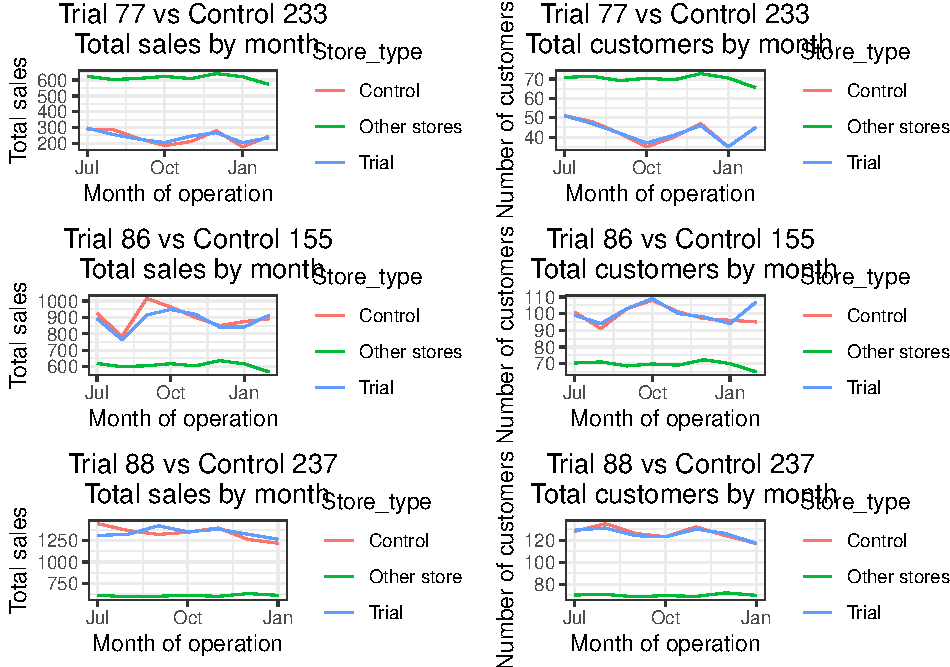
\includegraphics{Task2_files/figure-latex/unnamed-chunk-18-1.pdf}

\end{document}
